\section{Introduction}
% \todo{Cut most of this.}
%
% From the point of view of cross-linguistic typology, most sound systems are phonetically natural, and most sound changes are too \citep{Garrett2013}.
%
\todo{Most classes are natural, but not all natural classes are equal; some seem to be much rarer than others. Trying to understand why things are this way should be caused (in whole or in part) by the trajectory of regular sound change, cite refs. and discuss EP vs PBP in a couple of lines. Implicit in dominant accounts of the conditioning of sound change (and the predictions about its typology) is the idea that the different environments in which a new phonological rule arises should constitute (equally?) good phonetic precursors for it. Fruehwald talks about cases in which we don't necessarily expect this to be the case; we argue here that not only is it not the case, but that even in cases which look like they have some representational unity ([sonorant]), not all precursors seem to work; the mismatch between poor cue strength and abstract representational relationship to the original triggering environment gives us both a cue to the early phonological conditioning of regular phonetic change, and a probabilistic prediction about the relative frequency of certain kinds of representationally-coherent class. Clue about phonological conditioning also lies in the fact that it's hard to 'stop at' sonorant — once you get there, you often extend further.}.

\todo{further implicit in this argument is that we are talking about the end-products of sound change (blevins, RBO, frueh) and not the 'elaboration of' (read FR paper). if we're really talking about 'elaboration of', then we need some explicit theory of what that set can contain; argue that it is ambiguous whether we should see this representational control as 'end product' or 'further elaboration', but clear that it happens.}

look at this super cool empirical data we found

this tells us that bad phonetic cues + good abstract relationship = rare natural class


so this article also fills a gap in both synchronic natural class typology and in the typology of the conditioning of sound change

%
% The problem of naturalness is related to the well-known problem of the degree of phonetic regularity in sound change. How closely must the trajectory of a sound change correspond to the predictions we would make based on the physical properties of the human sound system? \todo{Heavily condense this, instantiate a couple of lines of the old naturalness thing.}
%
% Consider a phonological process P triggered by the set of \emph{front vowels}, \{i e\}. If the process is, say, \emph{palatalisation} in a following consonant, then we can argue that each of these vowels constitutes a sensible phonetic trigger, of broadly similar strength. If the process is instead \emph{devoicing} or \emph{nasalisation}, then this is not the case: devoicing and nasalisation are common operations, and may be perfectly natural in certain environments, but are not at all phonetically promoted by \{i e\}. There is then a sense in which the palatalising alternation is more (synchronically) natural than the nasalising one, even though both involve the same \emph{natural active class} of triggering segments. Most models of sound change then end up converging on the prediction that front-vowel-triggered palatalisation is more likely to emerge in any given language than front-vowel-triggered nasalisation. Certain accounts in which the mechanism of change is largely extra-grammatical and solely arises from the accumulation of production-perception interactions---an obvious example is \cite{Ohala1981}'s \emph{hypocorrection}, but see also the error accumulation model of \cite{Baker2011}---also make the \emph{stronger} prediction that change in each individual environment must be directly proportional to the strength of that environment as a phonetic precursor to change\footnote{This is a point originally made by \cite{Fruehwald2016}. Let's posit a case in which a continuous phonetic parameter $p$ is subject to change in a set $S=\{s_1,s_2\}$ of segmental conditioning environments (in which there are functionally-grounded reasons for $p$ to vary). If $s_1$ has a `stronger' phonetic-perceptual effect than $s_2$ (e.g. exerts a greater coarticulatory effect on a preceding segment), then the bias toward change in $s_1$-contexts is greater than the bias toward change in $s_2$-contexts. Over time, this accumulates, and $s_1$ corresponds to both a greater rate of change, and a more divergent realisation.}. This is really an extension of the argument about palatalisation and nasalisation above: if class A can be `better' with respect to a particular alternation than class B, it is also almost certainly the case that one individual member of class A /a$_1$/ can be, in itself, a better trigger than another segment /a$_2$/ also in A.
%
% Three suggestions underlie the remainder of this discussion. The first is that there is a wide typology of what I'll call less-natural classes, ranging from the most disjoint `Evenki'-like cases, to `mostly-natural' classes: L-shaped classes that can be described as the \emph{union} of a straightforwardly-natural class and an external, but related object. In itself, this is not new---disjunctively-specified environments are often posited (\citealt{Flemming2005} for counterarguments); but the problem of whether such classes have an independent reality (rather than being emergent from conspiracies of constraints) is an open one. The second central suggestion is that there is a relationship between the structure of active classes, and the pathways by which phonological change proceeds: L-shaped classes arise as a sensible consequence of rule-extension during the phonologisation of (that is, the incorporation into the synchronic grammar of) a sound change, and reflect in their organisation the metric by which such extensions are evaluated and updated. One of the conjectures that we make in this paper is that \emph{if} the shape of an active class is not overdetermined by multiple properties of the language (that is: if the language already contains mismatches between acoustics, perception, and representation), then recourse is made to the most abstract tier of information available; this raises a further problem of discrimination that we consider briefly below. Finally, we argue that we need more than phonetic precursors in the explanation of phonological generalisations; the selection of the set of segments involved in the innovated pattern considered throughout this paper is best understood as categorical and phonological.
%
% \subsection{this paper}
%
% The relationship of this paper to the overarching structure of this thesis is in the notion of similarity-driven change considered. We suggested that the similarity of the final target set to an initial, functionally well-motivated segmental trigger drove the variable phonologisation of Turkic onset obstruentisation in \cref{chapter:deson}, and underlies (whether synchronically or diachronically) the typology of sonorant-sonorant assimilations considered in \cref{chapter:nl}. In this paper, we deal in slightly greater depth with the issue of what we expect to see when phonologisation is `driven' by some parameter, and of how the synchronically-active class associated with a phonological pattern is regularised. The case considered is a recent phonological innovation in Turkish, not previously addressed in the phonological literature, targeting the mid vowels /e, ø/ in closed syllables; much of the empirical substance of this paper is devoted to the presentation of experimental results relating to this case.  A drastic and categorical lowering of /e/ and a less-drastic lowering of /\o/ in syllables closed by [+sonorant] segments or the voiced fricative /z/ can be analysed as a set of successive generalisations, beginning in /e/ and spreading to /\o/, which is further behind in the change.
%
The major subsidiary goal of this paper is incremental empirical progress with respect to the phonology of modern Turkish. Although the cases of vowel harmony and of anomalous stress in Turkish are familiar to almost all phonologists, little attestation of the novel pattern we report here exists in the descriptive literature on Turkish, and none at all in the phonological literature. We argue that the current study fills a gap both in the state of language-specific knowledge, and more generally in the broad typology of the end-products of sound change.

this paper is organised as follows.
% \Cref{s:naturalclasses} contains a preliminary discussion of some illustrative examples from Swiss German dialects (\cref{ss:schaffhausen}) and Georgian (\cref{ss:georgian}), with reference to the problem of class formation.
In \cref{s:turkishcase}, we introduce the innovation in Turkish on which the rest of this paper \ focuses; \cref{ss:dialectology} discusses the similar but non-identical patterns that arise in non-standard varieties of Turkish, and \cref{ss:coda_effects} provides the broader context of the typology of closed-syllable height effects. \Cref{s:methods} contains a straightforward overview of the setup, methodology, and sampling of the study on which the remainder of the chapter is based. The acoustic data are addressed throughout \cref{s:trdata}; \cref{ss:distrib} deals with the overall distribution of results and the categoricity of the Turkish pattern, and \cref{ss:tr_codas} considers the details of the behaviour of individual segments. We treat the various classes of exceptions to the alternation in \cref{ss:trexceptions}, and provide the overall perspective from the point of view of the hypothesised diachrony in \cref{s:tr_diachrony}, along with some recapitulation of the state of inter-speaker variation and the typology in \cref{ss:trvariation}.

\clearpage
\section{Pre-sonorant mid vowel lowering in Turkish}\label{s:turkishcase}

In this section, we set out the case that the remainder of this study will investigate in detail; a note refreshing the reader's memory of well-known features of the Turkish phonological system is given in \cref{sss:trphonology}, the pattern itself is described in \cref{ss:trcase}, and \cref{ss:trstudy} briefly motivates the experimental work whose setup and methodology appear in \cref{s:methods}. Detailed experimental results follow in \cref{s:trdata}.

\subsection{Notes on the overall system}\label{sss:trphonology}
For the reader's reference, we briefly contextualise the discussion with an overview of salient features of the Turkish phonological system. Turkish is generally understood in the phonological literature to have eight contrastive vowels (\citealt{Hulst1991}, \citealt{Kabak2011}), whose phonological behaviour is well-known (for overview, \citealt{Clements1982,Kabak2011}): processes of backness and rounding harmony both operate left-to-right across roots and suffixes, under the systematic constraint that rounding may only spread to high vowels in non-initial syllables. Although all eight vowels in the system are paired for backness and roundness, it is therefore the case that a gap arises in the non-initial syllables (\cref{fig:trvowelsall}) – the rounded mid vowels do not appear in these positions, save in loanwords. /e/ is therefore the only non-high front vowel that may appear in any position in the word, and the only vowel outside initial syllables that we can see as having `room' to vary freely in height---/i/, /y/, /ɯ/, /u/, and /ɑ/ are all constrained in one direction by the ceiling or the floor of the vowel space. The alternation in \cref{ex:trson} then looks like the right-hand diagram in  \cref{fig:trvowelsall}: pre-sonorant realisations of /e/ and /ø/ \emph{fill a gap} along the front diagonal of the vowel space. \\

\begin{figure}[H]
  \centering
 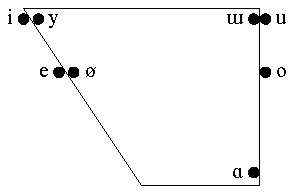
\includegraphics[width=0.32\linewidth]{tikz_vowels1}\hfill  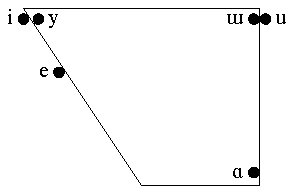
\includegraphics[width=0.32\linewidth]{tikz_vowels2} \hfill  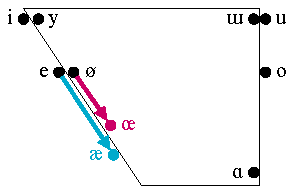
\includegraphics[width=0.33\linewidth]{tikz_vowels3}
\caption{Turkish vowels in initial syllables (left) and in non-initial syllables (center); sonorant-conditioned alternations shown in the Turkish vowel space (right).}
\label{fig:trvowelsall}
\end{figure}

The majority of the Turkic languages share similar systems of backness harmony, and most extend this to an allophonic distribution of \emph{consonantal} segments (most strikingly in Karaim, in which the typical system of [back]-spreading appears to have been lost for the vowels, and retained instead as long-distance consonant harmony; \citealt{Nevins2003}). \cite{Clements1982} describe the Turkish velars /k, g/ and the lateral /l/ as being typically [+back] in the context of [+back] vowels and [-back] in the context of [-back] vowels, although subject to various blocking effects and lexicalised exceptions. We consider (although not in exhaustive depth) the state of phonetic data on the backness of the lateral /l/ in \cref{sss:lateral} below, with respect of the potential for degree of palatalisation to affect the lateral's suitability as a phonetic precursor to vowel-lowering; the experimental data conform well to the characterisation here.

The remainder of the sonorants are not, as far as the literature is aware, subject to alternations of this particular type, although the rhotic has variable realisation in general; it may be tapped, trilled, or approximant, and may be fricated, devoiced, or entirely deleted (the latter particularly in the imperfective /–iyor/ and the indefinite article /bir/). The literature is rather variable as to the state of the rhotic; although accounts generally coincide \citep{Lewis1967,Goksel2005} in describing it as either an alveolar tap or trill, accounts of the extent to which it is subject to frication and devoicing vary. \citet[p.~7]{Lewis1967} and \citet[p.~29]{Kopkalli1993} claim that devoicing and frication are exclusively word-final, contradicting \citeauthor{Blaskovics1964}'s (\citeyear[p.~5–10]{Blaskovics1964}) description of front-vowel-dependent frication in the rhotic. \cite{Comrie1997Tr} describes rhotic frication as exclusively \emph{word-initial}; \citet[p.~25]{Yavuz2011} claim that frication applies both word-initially and word-finally, but that devoicing is restricted to the word-final position. Due to the general constraints of experimentation, we make no strong claim here as to the status of the rhotic, other than the establishment of its broad tendency towards strongly devoiced realisation. Impressionistically, in our sample, all utterance-final rhotics were voiceless and fricative in realisation; intervocalic and pre-consonantal rhotics were generally flapped (although occasionally trilled, assimilated to an adjacent lateral, or approximant).

\subsection{The case}\label{ss:trcase}

In Turkish, the front mid vowels /e/ and \ur{\o} undergo alternations conditioned by the following coda, summarised ultimately (with reference to the results and descriptive discussion that follow in \cref{s:trdata}) in \cref{ex:trson,ex:trresyll,ex:trother} below---/e/ and \ur{\o} are systematically low in a syllable closed by a sonorant, and /e/ is (for many speakers, but subject to significant inter-speaker variation; \cref{ss:trvariation}) slightly raised relative to the non-sonorant mean in either pre-obstruent contexts, or in contexts in which the coarticulatory effect of high vowels is particularly significant. We focus in this paper \ particularly on the state of /e/, which is more frequent in the lexicon and displays more clearly categorical and phonetically discontinuous behaviour. \Cref{ex:trresyll} is illustrated in \cref{fig:trwords} with data from the study in \cref{s:trdata} for \textbf{one} representative (F09; female, b. 1980 Ankara) speaker. Pre-sonorant /e/ in un-affixed forms has F1 in the range 750–900 Hz; the corresponding alternant /e/ post-resyllabification has F1 400–600 Hz.

\begin{example}\label{ex:trson}
/e/ and \ur{\o} surface as [\ae \ $\sim$ a] and [\oe] respectively in sonorant-closed syllables:
  \begin{tabbing}
      \ur{erdem} \tab[2cm] \= [ær.dæm] \tab[3cm] \=`virtue' \\
      \ur{hejkel} \> [hej.kæl] \>`statue' \\
      \ur{gizem} \> [gi.zæm] \>`mystery' \\
      \ur{biber} \> [bi.b\ae r] \>`pepper' \\
      \ur{g\o l} \> [g\oe l] \>`lake'\\
      \ur{g\o m-mek} \> [g\oe m.mek] \>`bury-{\sc\scriptsize INF}'
  \end{tabbing}
\end{example}

\begin{example}\label{ex:trz}
And, for some speakers, in syllables closed with /z/:
  \begin{tabbing}
      \ur{pekmez} \tab[2cm] \= [pek.mæz] \tab[3cm] \=`treacle' \\
      \ur{merkez} \> [mær.kez] $>$ [mær.kæz] \>`center' \\
      \ur{gel-mez} \> [gæl.mæz] \>`does not go'
  \end{tabbing}
\end{example}

\begin{example}\label{ex:trresyll}
Affixation destroys the environment for lowering (\cref{fig:trwords}):
  \begin{tabbing}
      \ur{erdem-i} \tab[2cm] \= [ær.de.mi] \tab[3cm] \=`virtue-{\sc\scriptsize ACC}' \\
      \ur{hejkel-im} \> [hej.ke.lim] \>`statue-{\sc\scriptsize 1SG.POSS}' \\
      \ur{gizem-in} \> [gi.ze.min] \>`mystery-{\sc\scriptsize GEN}'\\
      \ur{biber-in} \> [bi.be.rin] \>`pepper-{\sc\scriptsize GEN}'\\
      \ur{g\o l-i} \> [g\o .ly] \>`lake-{\sc\scriptsize ACC}'\\
      \ur{g\o m-er} \> [g\o .m\ae r] \>`bury-{\sc\scriptsize 3SG.P}'
  \end{tabbing}
\end{example}

\begin{example}\label{ex:trother}
No lowering in other environments; some speakers show pre-obstruent /e/-raising:
  \begin{tabbing}
      \ur{dede} \tab[2cm] \= [de.de] \tab[3cm] \=`grandfather' \\
      \ur{bebek} \> [be.bek] $\sim$ [be.be̝k] \>`baby' \\
      \ur{herkes} \> [h\ae r.kes] $\sim$ [h\ae r.ke̝s] \>`everybody'\\
      \ur{taze} \> [ta.ze] \>`fresh'
  \end{tabbing}
\end{example}

\begin{example}\label{ex:trheightharmony}
Unstressed open syllables preceding high vowels /i, y/: /e/ raised (\cref{sss:coarticulation}).
  \begin{tabbing}
      \ur{deniz} \tab[2cm] \= [dɪ.niz] \tab[3cm] \=`sea' \\
      \ur{kedi} \> [kɪ.di] \>`cat' \\
      \ur{be-nim} \> [bɪ.nim] \>`my'
  \end{tabbing}
\end{example}

\begin{figure}[H]
  \centering
  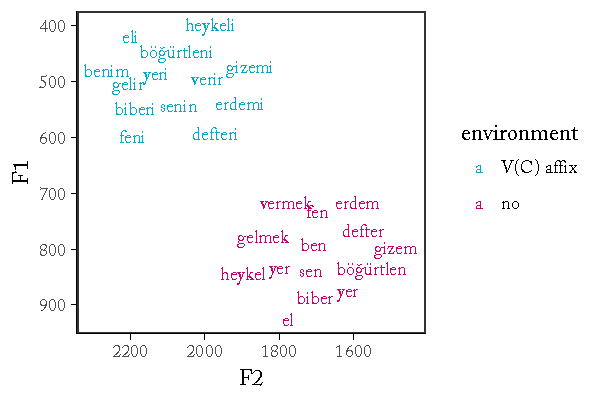
\includegraphics[width=0.48\linewidth]{tr_osen_words}\hfill
    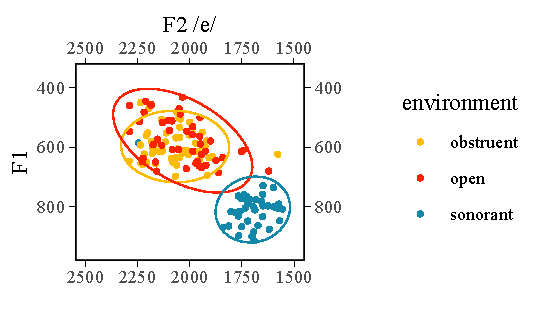
\includegraphics[width=0.48\linewidth]{tr_osen_vowels}
  \caption[pre-sonorant {\it heykel, sen, biber \ldots} vs. affixed pre-vocalic {\it heykel-i, sen-in, biber-i \ldots}]{F09: F1/F2 space (Hz) for alternating /e/. Let, pre-son. unaffixed {\it b\textcolor{todo}{e}n, bib\textcolor{todo}{e}r, böğürtl\textcolor{todo}{e}n, deft\textcolor{todo}{e}r, \textcolor{todo}{e}l, erd\textcolor{todo}{e}m, f\textcolor{todo}{e}n, giz\textcolor{todo}{e}m, heyk\textcolor{todo}{e}l, s\textcolor{todo}{e}n, y\textcolor{todo}{e}r} \& C-initial suffixed {\it v\textcolor{link}{e}rmek, g\textcolor{link}{e}lmek} vs. pre-vocalic {\it b\textcolor{link}{e}nim, bib\textcolor{link}{e}ri, böğürtl\textcolor{link}{e}ni, deft\textcolor{link}{e}ri, \textcolor{link}{e}li, erd\textcolor{link}{e}mi, f\textcolor{link}{e}ni, g\textcolor{link}{e}lir, giz\textcolor{link}{e}mi, heyk\textcolor{link}{e}li, s\textcolor{link}{e}nin, v\textcolor{link}{e}rir, y\textcolor{link}{e}ri}. Right, all measurements coded by environment, 95\% confidence ellipses.}
  \label{fig:trwords}
\end{figure}

We are not aware of any reference to this set of alternations in the formal phonological literature. Several general descriptions of the language are available, and vary in their characterisations of the system, in a manner consistent with the suggestion that the pattern under consideration is a recent development in Turkish. \citeauthor{Lewis1967}'s\ (\citeyear[14]{Lewis1967}) reference grammar describes raising in unstressed open syllables: `a closer pronunciation, verging on the sound of {\bf i}, especially in the first syllables of [\ldots] {\bf gece} `night' ', but mentions no lower allophone and no preconsonantal effects of any kind. \citet[512]{Kornfilt1997}, 30 years later, claims that an `alternation phenomenon affects the front, non-high vowel [e] and [ø], which are lowered before sonorants in closed syllables'; she transcribes the lower allophone of [e] as [ɛ], although it's unclear to what extent this decision is impressionistic (or informed by real phonetic properties). \citet{Goksel2005} give the distribution of /e/ as [æ] before sonorants, [ɛ] in stressed open syllables, and [e] elsewhere. We argue that none of these characterisations adequately represents the state of the system as we find it in current data, with the note that the disparity in descriptions corresponds to a significant time-separation and is concordant with further discussion of the relative recency of this pattern. In \cref{s:trdata}, we present the production-study results that support the characterisation we propose in \cref{ex:trson,ex:trresyll,ex:trother,ex:trheightharmony}.



\subsection{Coda-triggered height effects}\label{ss:coda_effects}

The descriptive case(s) in Turkish that constitutes the majority of this paper \ can be placed at the intersection of two larger typologies of phonetically well-motivated phenomena: one of vowel quality effects conditioned by syllable structure, and the other of height effects triggered, irrespective of syllabic considerations, by the various sonorant segments. The pattern in Turkish  either of these typologies: while closed-syllable vowel laxing is well-established, it is rarely predicated on the manner of articulation of the coda involved; and while rhotic-triggered height effects are common, they are rarely extended to the set of all sonorants and rarely dependent on syllable structure.

\subsubsection{Closed-syllable vowel laxing}\label{sss:csvl}

It is reasonably well-established that there exists a general cross-linguistic tendency towards laxer vowels in closed syllables and tenser vowels in open syllables, both in distribution and in allophonic patterning; a straightforward example is the alternation that appears in French \emph{nous gavottons} [nu ɡa.vo.tɔ̃] `we gavotte' and \emph{rigolo} [ʁi.go.lo] `funny (masc.)', but \emph{il gavotte} [il ga.vɔt] `he gavottes' and \emph{rigolote} [ʁi.go.lɔt] `funny (fem.)'. \citet[p.~223–226]{Storme2017PhD} gives a non-exhaustive but substantial typological survey of 18 languages in which some such generalisation holds; for all these cases, `lax' is understood acoustically to imply a two-dimensional movement in the vowel space, with a lax vowel having less peripheral F1 and F2 targets than a tense counterpart. Not all attested cases are equally general; in some languages laxing applies across the board to all vowels in closed syllables, while in others further restrictions on the affected vowel\footnote{e.g.~\citet{Nordhoff2009}: Sri Lanka Malay has the five-vowel inventory /a e we o u/, but only /e o/ alternate.} or the consonantal context apply (\cref{tr:csvl_specific}). It is unclear whether apparent statistical tendencies should be expected to hold more broadly or carry particular significance. If we were to take \citeauthor{Storme2017PhD}'s survey as broadly representative, we would observe that the mid vowels /e o/ are slightly under-targeted\footnote{Although available in all surveyed inventories but one, /e o/ undergo laxing in 7 of 17 languages; French (Southern), Chamorro, Indonesian, Kairiru, Paluai, Sri Lanka Malay, Kuteb. The remaining languages surveyed target exclusively the more peripheral vowels, particularly /i u/.}, and that languages invoking segment-specific constraints do so particularly with respect to rhotics and dorsals\footnote{Patterns of the uneven distribution of vowel height in the context of uvulars and velars are well-known; for an overview, see \citet[p.~103]{Gallagher2016}.}.

\begin{example} \label{tr:csvl_specific}
  \textsc{(Uma Juman) Kayan} (Austronesian, Borneo): high vowels are lowered if followed by /h, l, r, ʔ/. \citep[p.~263]{Blust2013}
  \begin{tabbing}
  \ur{lakiʔ} \tab[2cm] \= [lakeʔ] \tab[2cm] \= `male'\\
  \ur{uruʔ} \> [uroʔ] \> `grass'\\
  \ur{hivih} \> [ˈhi.veh] \> `lower lip'\\
  \ur{duh} \> [doh] \> `female'\\
  \ur{bakul} \> [ˈba.kol] \> `basket'\\
  \ur{tumiɾ} \> [ˈtu.meɾ] \> `heel'\\
  \ur{ʔatuɾ} \> [ˈ{ʔ}a.toɾ] \> `arrange'
    \end{tabbing}
\end{example}

The existence of coda-conditioned effects on height and backness has been attributed in various cases \citep{Fery2003,Botma2012} to the existence of a close relationship between length, quality, and syllable structure; that is, contingent on the claim that vowels are shorter in closed syllables than in open syllables, which see e.g. \citet{Maddieson1985}. The duration-sensitive account of closed-syllable laxing then admits a connection to those patterns in which syllabically-conditioned length alternations arise, as \cref{tr:ingush}; but requires some form of the claim that longer vowels are tenser than shorter vowels.

\begin{example} \label{tr:ingush}
  \textsc{Ingush} (Nakh-Dagestanian, Ingushetia): underlying long vowels alternate with short vowels in closed syllables; short vowels don't alternate. \citep{Nichols2011}
  \begin{tabbing}
  \ur{duucə} \tab[2cm] \= [duːcə] \tab[2cm] \= `narrate-{\sc\scriptsize INF}'\\
  \ur{duuc} \> [ducː] \> `narrate-{\sc\scriptsize PRS}'\\
  \ur{niisə} \> [niːsə] \> `straight'\\
  \ur{niis-lu} \> [nis.lu] \> `becomes straight'

    \end{tabbing}
\end{example}

One potential issue for explanations along these lines is that empirical generalisations about the relationship between quality and duration are variable, and difficult to straightforwardly align with the demands of articulation or the typology of laxing. The claim that closed-syllable laxing derives from the loss of duration in closed syllables requires that lax vowels be uniformly shorter than tense vowels; given a non-low vowel subject to laxing, we expect the lax counterpart to be lower than the tense one, and therefore must claim that higher vowels are longer than lower ones. However, it is in fact frequently the case across languages that the first formant correlates positively with duration, and that therefore height itself is inversely correlated with duration: that is, the lowest vowels (with the highest F1) are the longest vowels.

Claims to this effect appear both within-category and cross-category. If all other parameters are constant, \citet{Lehiste1970} suggests that low vowels are longer than high vowels across the board, and posits physiological reasons relating to the gestural duration of jaw-opening; similar effects have also been attributed to the closeness of the jaw position during high vowels to that expected during most consonants \citep{Maddieson1997,Gussenhoven2007}. One of the more widely-known experimental results to this effect is \cite{Lindblom1963}'s claim that the F1 of Swedish non-high vowels decreases (that is, vowel height increases) exponentially as vowel duration decreases. Similar correlations are reported in English \citep{Peterson1960,Westbury1980}, Hindi \citep{Ohala1992}; and cf. \citet{Toivonen2015} for English and Swedish, and for a review of the literature. The relationship between duration and vowel height is revisited in \cref{sss:coarticulation,ss:trduration}. A portion of \citet{Storme2017ms,Storme2017,Storme2017PhD}'s argument for a new account rooted in the perceptually-driven enhancement of post-vocalic contrasts between consonants is predicated on the claim, as above, that the derivation of lowering and centralising effects from the loss of duration is not justified; a full treatment of this account and its relationship to the case we consider here is beyond the scope of this paper.

The essential relationship of the Turkish case to the cross-linguistic pattern is largely straightforward, although in a few respects particularly divergent; the pattern in Turkish appears to show a larger deviation in phonetic space than the typical case of closed-syllable laxing, as should become apparent from the experimental data presented below, and the class of segments targeted is a new one. We argue that the pattern in Turkish is \emph{lowering} rather than \emph{lowering plus centralisation}, and that any apparent centralisation arises solely due to the inherent topology of the vowel space; unlike \citet[p.~95]{Storme2017PhD}'s case in French, for which F2 effects appear to be too large to be accounted for by height targets alone.

\subsubsection{Sonorant-related height effects}\label{sss:tr_son_effects}

Sonorant-triggered---particularly, rhotic-triggered---height effects are fairly well-attested cross-linguistically, both as non-contrastive differences in the contextual distribution of formant values in phonetic space, and as apparent phonotactics. What distinguishes the latter `phonological' set from the patterns described in the previous section is the frequent absence of any restrictions relating to syllable structure; several cases of sonorant-conditioned laxing or lowering apply irrespective of the relative position of the sonorant trigger and the affected vowel. In the Austronesian language Thao \citep[p.~264]{Blust2013}, all high vowels lower if adjacent to the alveolar flap /ɾ/ \cref{tr:thao}; the requirement for adjacency applies in both tautosyllabic and heterosyllabic contexts, and the flap may precede or follow the affected vowel. (A further, more general case of laxing applies in the familiar set of closed-syllable environments.)

\begin{example} \label{tr:thao}
  \textsc{Thao} (Austronesian; Taiwan): high vowels lower\footnote{Also if adjacent to /q/: /tuqris/ [ˈtoq.ɾes] `noose trap', /qusaz/ [ˈqo.sað] `rain'.} adjacent to a rhotic. \citep{Blust2013}
  \begin{tabbing}
  \ur{ɾima} \tab[2cm] \= [ˈ{ɾ}e.ma] \tab[2cm] \= `five'\\
  \ur{ɾusaw} \> [ˈ{ɾ}o.saw] \> `fish'\\
  \ur{i{ɾ}uʃ} \> [ˈi.{ɾ}oʃ] \> `saliva'\\
  \ur{ɬmiɾ} \> [ɬmeɾ] \> `grass, weeds' \\
  \ur{tuɾu} \> [ˈto.ɾo] \> `three' \\
  \ur{hibuɾin} \> [hiʔ.bo.ɾεn] \> `be mixed together'
    \end{tabbing}
\end{example}

% rewrite if you have time
In general, throughout the phonetically-informed literature, attestation exists of significant effects in F1 conditioned by the presence of an adjacent sonorant. These vary between (what we would diagnose as) the `phonetic' and the `phonological' in their scope, and in which sonorants they involve. What seems broadly uncontroversial is that strong articulatory and acoustic properties of \defs{the rhotics} often favour the development of height effects in a pre-rhotic vowel. The most widely-cited acoustic characteristic of rhoticity as a whole is the lowered third formant \citep{Ladefoged2003}; but see \citet{Lindau1985} for complications. \Cref{fig:tr_rhotic_spectrum} shows spectra for a [ir]$\sim$[iʃ] pair in Turkish, for which there is a small but significant effect of the utterance-final rhotic on the preceding high vowel. The trill in particular \citep{Recasens1991,Recasens1999,Sole2002} has been shown to force tongue dorsum lowering and retraction, which \citet{Proctor2009} suggests (for Latin American Spanish) is a more general property of the whole class of coronal liquids. \citet{Bradley2010}, in a survey of Ibero-Romance, claims---unlike our case---that the effect of the post-vocalic trill on the height of the preceding vowel is strongest in the \textunderscore rV context, and weaker in \textunderscore rC, and attributes this to constraints on articulatory organisation.

\begin{figure}[h]
  \centering

  { \textit{bir} [bir̥] `one' \hfill \textit{diş} [diʃ] `tooth' }

  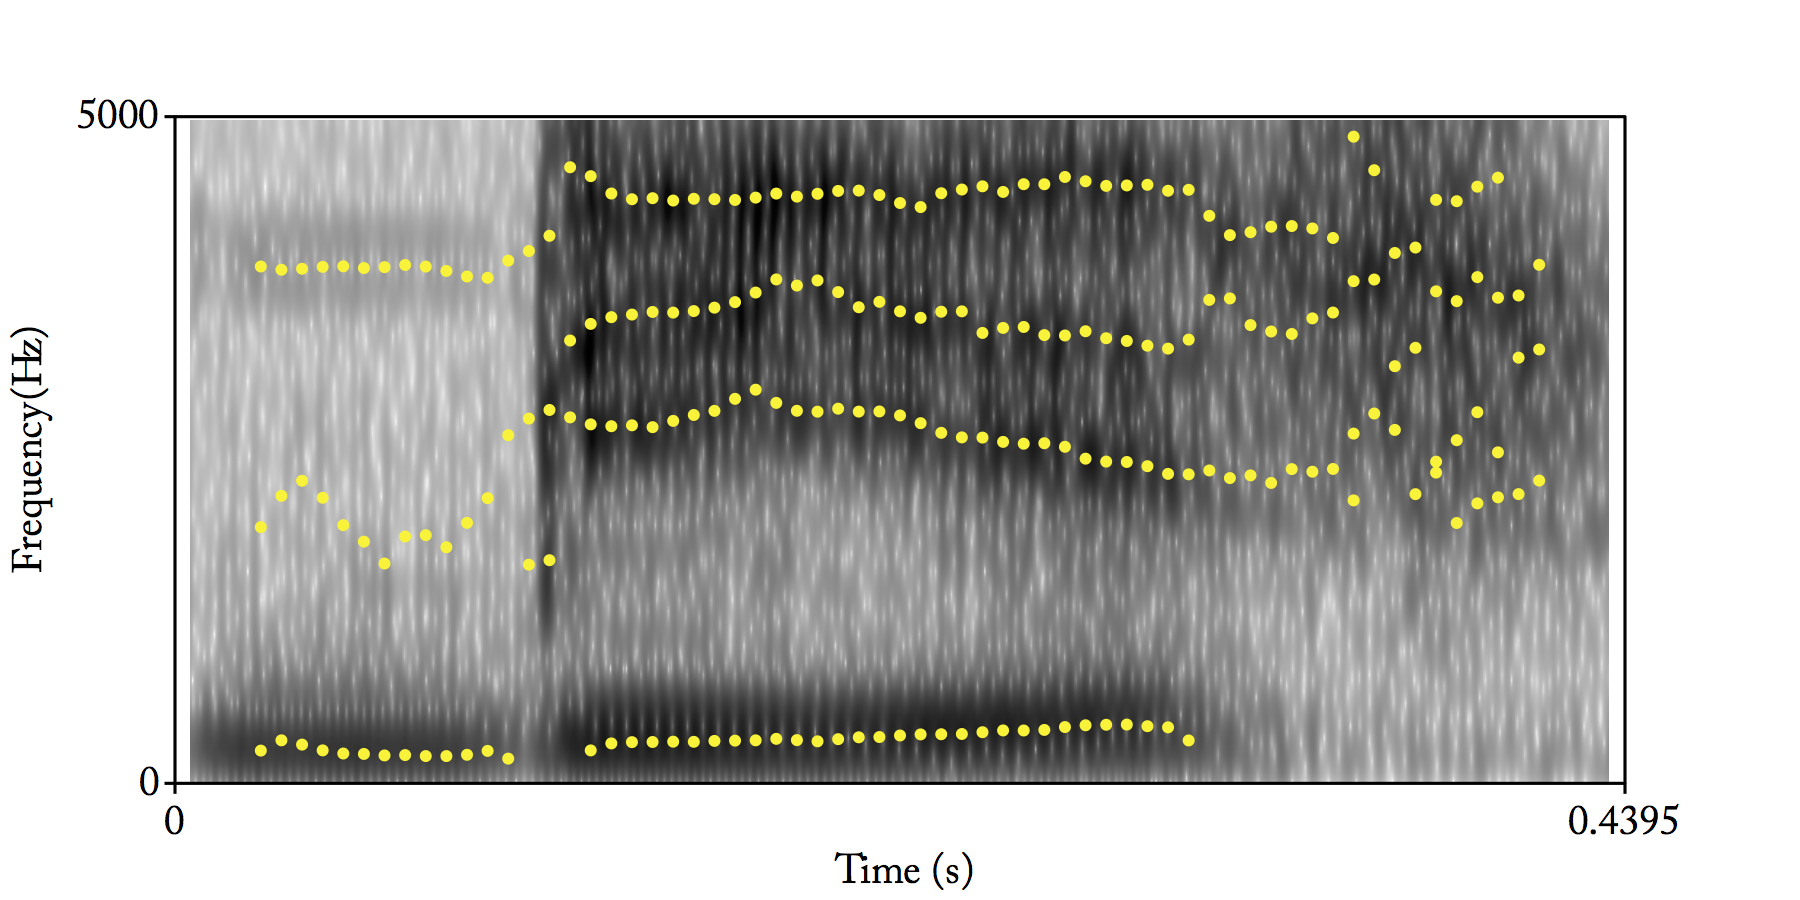
\includegraphics[width=0.45\linewidth]{tr_elif_bir.png}\hfill
  \includegraphics[width=0.45\linewidth]{tr_elif_diş.png}
  \caption[Spectrum for \textit{bir} `one' and \textit{diş} `tooth'.]{For one speaker (F01, Istanbul/1997), spectra with formants indicated for \emph{bir} [bir̥] `one' and \textit{diş} [diʃ] `tooth', showing formant movement driven by the presence of the rhotic.\footnotemark.}
  \label{fig:tr_rhotic_spectrum}
\end{figure}

\footnotetext{This is an utterance-final token; the rhotic is quite fricated.}

Mid vowel lowering before a rhotic coda is attested widely: throughout Ibero-Romance \citep{Bradley2010}, and in the context of the French \textit{loi de position} \citep{Storme2017}; in Swedish for /ɛ/ and /ø/ \citep{Riad2014}, in Faroese /e/ \citep{Arnason1999}, and, as before, in the examples for Schaffhausen German that we give in \cref{ss:schaffhausen}.
% A very incomplete typology of cases of this type appears in \cref{tab:tr_allcases}.
A detailed discussion of the situation of \defs{the laterals} appears in \cref{sss:lateral}, and we reserve a fuller overview for those passages. We draw particular attention to accounts of disparities between the rhotics and the laterals in degree and even direction of F1-effect; \cite{West1999} gives, for southern British English, significantly higher F1 in rhotic contexts than in lateral ones, and attendantly the prediction that lateral-triggered lowering effects should, in phonetically-controlled cases, be smaller; but note that this lateral is necessarily, due to the well-known state of English phonotactics, a velarised or `dark' one. Phonetically non-velarised laterals are often ignored by vowel-lowering rules, even after further generalisations and extensions (as with the case for Schaffhausen German given in \cref{ss:schaffhausen}); we therefore consider the state of the Turkish lateral in \cref{sss:lateral}.

In European Portuguese, \citet[p.~86--88]{Vigario2002} describes a fairly similar rule; the non-high vowels /e o/ must lower in word-final, unstressed syllables closed by a sonorant\footnote{Not in non-final syllables: \textit{revertér} [ʁɨ.vɨɾ.ˈtɛɾ] *[ʁɨ.vɛɾ.ˈtɛɾ]; except for /l/, which can trigger neutralisation across the board: \textit{delgádo} [dɛɫ.ˈga.du] `thin', \textit{relvínha} [ʁɛɫ.ˈvi.ɲɐ] `grass.\textsc{\footnotesize dim}'.} (the rhotic, the (velarised) lateral, or the nasals/nasal vowels), neutralising the contrast in /e o/–/ɛ ɔ/ and overriding the output of a general process that forces the raising of low vowels pre-nasal. Thus\footnote{\citet{Vigario2002} gives the relevant vowel only; all errors in the remainder of the IPA rendering here are mine.}, \textit{revólver} [ʁɨ.ˈvɔɫ.vɛɾ] `revolver', \textit{júnior} [ˈʒu.ni.ɔɾ] `junior', \textit{nível} [ˈni.vɛɫ] `level', \textit{álcool} [ˈaɫ.kɔɫ] `alcohol', \textit{sémen} [ˈsɛ.mɛn] *[ˈsɛ.mɨn] `semen', \textit{cólofon} [ˈkɔ.ɫu.fɔn] *[ˈkɔ.ɫu.fun] `colophon'. This reflects both a nice case of a similar alternation, and the (possible) phonologisation of the variable correlates of \defs{the nasals}:  although anticipatory nasalisation should drive an increase in F1 \citep{Krakow1988}, the introduction of the `nasal formant' \citep{Beddor1993,Beddor1986} drives a reduction in the perceptual space of the nasalised vowels, causing perceptual \textit{raising} in low-mid and low vowels. Where the Portuguese case differs from the Turkish one is in the systematic relationship to stress and plausibly therefore to duration, which we will revisit in \cref{ss:trduration}.
%
% \begin{table}[H]
% \centering
%   \begin{adjustbox}{width=\linewidth}
% \begin{tabular}{lll}
%   \toprule
% \textsc{Language} & Rule type & Triggers \\
% \midrule
% \bottomrule
% \end{tabular}
% \end{adjustbox}
% \caption[Sonorant-triggered height effects, across languages.]{A rough and incomplete typology of languages in which some form of sonorant-triggered height effect applies.}
% \label{tab:tr_allcases}
% \end{table}

\subsection{This study}\label{ss:trstudy}

In the preceding sections, we have addressed the extent to which we can coerce the Turkish pattern into a broader typology of patterns with seemingly similar phonetic and phonological conditioning. With the set of potential phonetic precursors in mind, we present below the results of our experimental investigation of the status of pre-consonantal height effects in the (standard) Turkish vowels, the evidence for their categoricity, and the details of their scope and conditioning.

One of the aims of this investigation is necessarily descriptive. We are not aware of a previous systematic investigation of height effects in Turkish vowels, or any formal analysis thereof; existing descriptions combine impressionistic auditory judgments and introspection, and as such require experimental confirmation. The experimentation described in the following section is a first approach to the descriptive problem; our discussion of the results in \cref{s:trdata} is framed around the issues of cross-linguistic typology and the phonetic precursors to phonologisation that we have raised in this section and in the introduction respectively.

\section{Methodology and sample}\label{s:methods}

All analysis that follows reflects data from a production study conducted between January 2016 and June 2017 in Manchester. Thirteen native speakers of Turkish, all resident at the time of experimentation in the UK, read a list of 220 items, along with a further list of 20 sentences containing target /e/ embedded in varied phonological and morphological environments. Speakers' ages ranged from 20-39; there were eleven female speakers and three male. All speakers were raised in the place of origin within Turkey (as listed in table \ref{tab:tr_metadata}); length of time resident outside Turkish-speaking areas ranged from 0.5 to 8 years. Speakers were not made aware of the purpose of the experiment prior to recording, and participation was voluntary---no payment was offered.

The preponderance of female speakers was an unfortunate artefact of the process of speaker recruitment. As such, more data is required to determine whether sex has a statistically meaningful predictive effect on the nature of the pattern, and we cannot comment further; we exclude data points corresponding to male participants from the overall statistical analysis and modeling, but these data are included in qualitative observations where appropriate.

\begin{table}[H]\setstretch{1.25}
  \centering\small
  \begin{tabular}{ccccccc}
      \toprule
      \textsc{ID} & \textsc{Year of birth} & \textsc{Place of origin} & \tab[1.5cm] & \textsc{ID} & \textsc{Year of birth} & \textsc{Place of origin} \\
      \midrule
      F01 & 1997 & Istanbul & & F08 & 1982 & Ankara \\
      F02 & 1995 & Istanbul & & F09 & 1981 & Istanbul \\
      F03 & 1991 & Istanbul & & F10 & 1980 & Ankara \\
      F04 & 1988 & Izmir & & F11 & 1978 & Ankara \\
      F05 & 1987 & Istanbul & & M01 & 1989 & Kayseri \\
      F06 & 1985 & Fethiye & & M02 & 1985 & Denizli \\
      \ F07 & 1983 & Bursa & & M03\footnotemark & 1980 & Kars\\







      \bottomrule
    \end{tabular}
  \caption{Speaker metadata (index, year of birth, region of origin) for all participants.}
  \label{tab:tr_metadata}
\end{table}

\footnotetext{Represents a fairly clear instance of dialectal divergence and excluded from overall calculations; see \cref{fig:abdiz} for discussion.}

\begin{figure}[h]
  \centering
  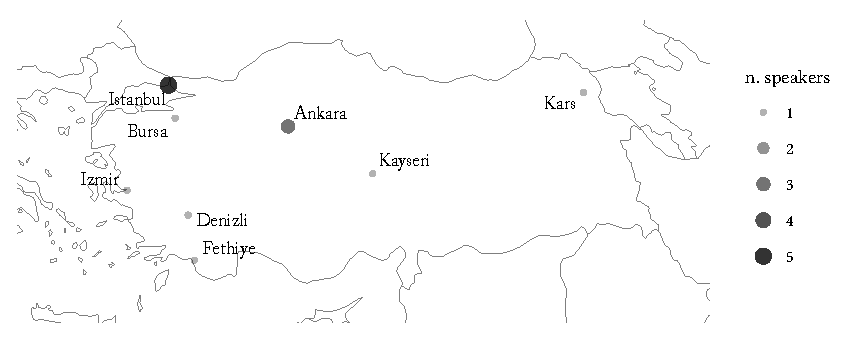
\includegraphics[width=0.90\linewidth,trim={5mm 10mm 5mm 0mm},clip]{tr_map}
  \caption[Map of participants' origins.]{Reference map of participants' origins\footnotemark.}
  \label{fig:trmap}
\end{figure}

\footnotetext{R: \texttt{ ggmap} \citep{ggmap}, \texttt{ ggalt} \citep{ggalt}.}

120 instances of /e/ appeared in the set of test items, in obstruent-closed (42), sonorant-closed (40), and open (38) syllables. 70 total were (primary-) stressed and the remainder unstressed\footnote{In practice, what this means is that these target vowels were in final and non-final syllables respectively: Turkish stress is typically word-final when regular, and although exceptionally-stressing items exist (on which \citealt{Inkelas1999, Kabak2001,Inkelas2003}, inter alia) these were not tested.}. The test set contained 32 instances of \ur{\o} (8 pre-obstruent and open; 16 pre-sonorant). Due to distributional restrictions on Turkish vowels, \ur{\o} almost never appears outside initial syllables, and is lower-frequency than /e/. The distribution of \ur{\o}-containing tokens was therefore necessarily particularly skewed with respect to stress---the pre-obstruent and pre-sonorant categories were evenly split, but all but one of the /\o/ in open syllables were unstressed: the French loan \textit{banliyö} `banlieue' was included, but not all speakers found it acceptable. The remaining items provided data on the non-target vowels. A full list of items tested is provided in the appendix, in the standard Turkish orthography with phonemic transcription and gloss; those expected to be exceptional have been marked.

\begin{table}[H]
\centering
\begin{tabular}{cccc}
  \toprule
\textsc{environment} & e & \o & \textsc{control} \\
\midrule
no coda & i.ˈl\textit{e} `with' & b\textit{\o}.ˈlym `chapter' & d\textit{a}.ki.ka `minute' \\
coda obstruent & ʃi.ka.j\textit{e}t `complaint' & ˈtʃ\textit{ø}p `garbage' & h\textit{a}s.ta `ill' \\
coda sonorant & bi.ˈb\textit{e}r `pepper' & \textit{ø}r.ˈnek `example' & sa.ˈm\textit{u}r `sable' \\
\bottomrule
\end{tabular}
\caption{Example items}
\label{tab:tr_wordlist}
\end{table}

For each speaker, one repetition of the wordlist and sentence-list was recorded. Recordings were made in a quiet room using a Sony PCM-M10 linear PCM recorder and an Audio-Technica ATR1200 cardioid microphone, and saved sampled at 44.1 kHz. Speakers were encouraged to read at a comfortable pace, and to correct themselves if unhappy with their own production. (120 stimuli + 20 sentence-internal targets)$*$(13 speakers) $=$ 1820 total instances of /e/ and 416 total instances of \ur{\o} were recorded, minus 13 \ur{\o} and 14 /e/ that occurred in lexical items that individual speakers found unacceptable. 55 /e/ tokens (3\%) were removed due to the diagnosis of systematic and conditioned exceptionality, and treated independently. 10 /e/ (0.55\%) and 19 \ur{\o} (4.6\%) of these were excluded due to deletion or devoicing, mispronunciation/production errors, segmentation difficulties, interference from non-modal voicing, and post-palatalisation coarticulation, leaving 1746 instances of /e/ and 383 instances of \ur{\o} for analysis. 2511 tokens were measured for the remaining 6 underlying vowels as comparison; since these were non-target vowels, no attempt was made to balance their distribution (/ɑ/ 843, /ɯ/ 258, /o/ 234, /i/ 560, /y/ 366, /u/ 250).

A further set of exploratory data were collected to test systematic patterns of exceptionality, representing a further 300 tokens of /e/. These were excluded from the overall statistical analysis, and were not distributed evenly among speakers: the state of this extra dataset is discussed in detail in subsection \ref{ss:trexceptions}.

All segmentation and acoustic analysis were carried out in \texttt{Praat} \citep{Praat}; target vowels were extracted from the produced tokens, with boundaries inserted manually based on visual inspection of the waveform and spectrogram. In pre-/post- obstruent and pre-pausal contexts, the beginning and end of the target vowel was established with a reasonable degree of confidence by the presence of low-frequency periodic noise and clearly-visible formant structure. For vowels post-sonorant, the initial boundary was placed at the onset of the formant steady-state. Pre-nasal, the appearance of the high-amplitude formants associated with a nasal release was abrupt enough to provide a high-confidence end boundary, but for laterals and rhotics the cues to the transition (formant values, intensity) are typically more gradual; pre-pausal \ur{r} showed significant frication, distinguishing it unambiguously from the target, and the final boundary pre-lateral was placed where a significant change in formant trajectory and intensity coincided.

F1 and F2 (in Hertz) were measured at 3 points (25\%, 50\%, and 75\% of inter-boundary duration) and averaged, and duration (in milliseconds) was automatically exported by a \texttt{Praat} script. All statistical analysis was done in R \citep{R}. Formant data were then normalised to formant-extrinsic $z$-scores (Lobanov-normalised; \citealt{Lobanov1971, Adank2004}) for comparison across speakers, using the R \texttt{ phonR} package \citep{phonR}.

\section{Data}\label{s:trdata}

In this section, we present the acoustic data relating to coda-conditioned height effects in Turkish. This begins (\cref{ss:distrib}) with a demonstration of the patterns's robustness and apparent phonological categoricity; \cref{ss:trduration} deals with the patterning and condition of vowel duration. Details of lexical exceptions and blocking environments appear in  \cref{ss:trexceptions}, individual triggering segments in \cref{ss:tr_codas}, and the (incipient) generalisation to some voiced obstruents is considered in \cref{sss:trvobst}.

Since the focus in this discussion is on the comparative state of the system rather than specific physical-acoustic properties for which a rescaling to a Hertz-like value might be of interest, we have presented the Lobanov-normalised/$z$-score measure directly, throughout. For /e/, the range of non-normalised F1 values is $[346.98,1178.94]$ (Hz), and of F2 values $[1136.88,2828.44]$; for /ø/, the F1 range is $[334.02, 851.42]$, and the F2 range is $[1062.01, 2329.58]$.

\subsection{Distribution and categoricity}\label{ss:distrib}

In \cref{fig:trwords}, we presented a sample of evidence that pre-sonorant /e/ in forms like unaffixed \emph{heykel} and affixed \emph{heykeli} shows distinct realisations. In this subsection, we demonstrate that these distinct, and distributionally discontinuous /e/-realisations correspond strictly to the nature of the following coda, and claim that this is indicative of a categorical, phonological effect targeting /e/ in syllables closed by a sonorant coda.

How do we diagnose a \emph{phonologically}-conditioned effect? The classical criterion that we implicitly cite in \cref{ex:trresyll,fig:trwords} is the existence of morphologically-sensitive \emph{alternation}; affixation destroys the environment for lowering. One straightforward approach when faced with unstructured empirical data is to search for bimodality in the acoustic signal: if some phonetic parameter P has a discontinuous distribution, the probability that P is subject to some phonological effect increases\footnote{For complications, cf.~\citet{Scobbie2005}: broadly, phonetic discontinuity signals categoricity, continuous distribution signals gradience; but this is subject to various confounds and empirical difficulties.}. Probability density functions\footnotemark (PDFs) on (Lobanov-normalised) F1 and F2 are given in figure \ref{fig:trdensity}, representing the distribution of all tokens of each `phonemic' vowel category in the experimental result; an idealised Gaussian distribution with identical mean and standard deviation has been overlaid to aid the reader's eye in assessing deviation from a normal model. F1 and F2 distributions for /e/ are strongly bimodal (i.e. have two local maxima); Hartigan's dip test indicates that the distribution of both parameters is not unimodal (strongly so for F1: $p$ 0.03597; weakly for F2: $p$ 0.08897).

\footnotetext{These and further PDFs following are calculated using `kernel density estimation' \citep{Silverman1986}, which {\it non-parametrically} estimates the probability density function for a random variable given a finitely-sized data sample: being unbound to any predetermined shape, kernel density estimates are better able to capture the presence or absence of irregularities in the distribution of data than parametric estimates. In base R: function \texttt{ density}; in \texttt{ ggplot2}: \texttt{ stat\_density}.}

\begin{figure}[H]
  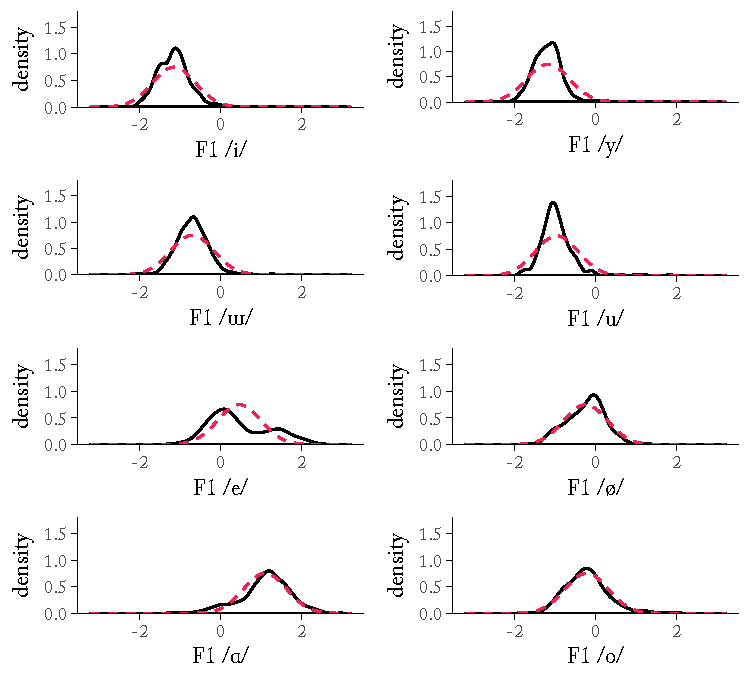
\includegraphics[width=0.49\linewidth]{tr_gaussian_density}
  \hfill
  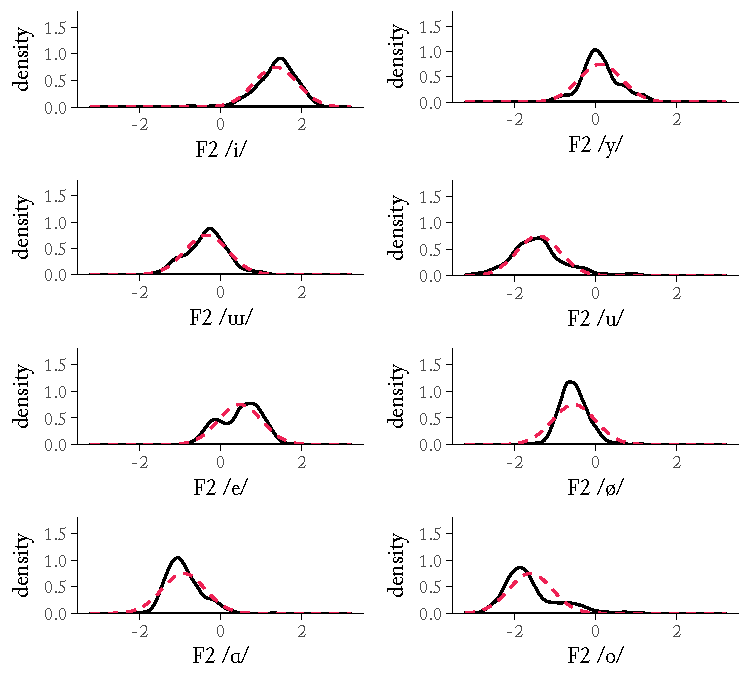
\includegraphics[width=0.49\linewidth]{tr_gaussian_density_F2}
  \caption[Probability density functions for F1 and F2, all categories.]{Probability density functions for F1 and F2, Lobanov-normalised across all speakers, in 8 vowel categories, with overlaid idealised Gaussian.}
  \label{fig:trdensity}
\end{figure}

Figure \ref{fig:trexploded} suggests that this bimodality derives from the composition of distinct distributions for the contextual realisations of /e/. If the sample is decomposed by context (syllable closed by {\it obstruent}, syllable closed by {\it sonorant}, open syllable), basis density functions can be calculated post-resampling whose maxima differ, but whose individual behaviour is no longer multimodal; the modes for these recalculated functions correspond to the multiple maxima in \cref{fig:trdensity}. The probability density function across all tokens for \ur{\o} shows no obvious bimodality on initial examination, but an apparent effect arises---especially in F1---on visual inspection when decomposed by context\footnote{The existence of multiple `real' modes in a sample can be masked by insufficient overall distance, as with the superposition of two normal distributions whose means differ by less than the sum of their standard deviations---see for overview \citealt{Schilling2002}}.

\begin{figure}[H]
  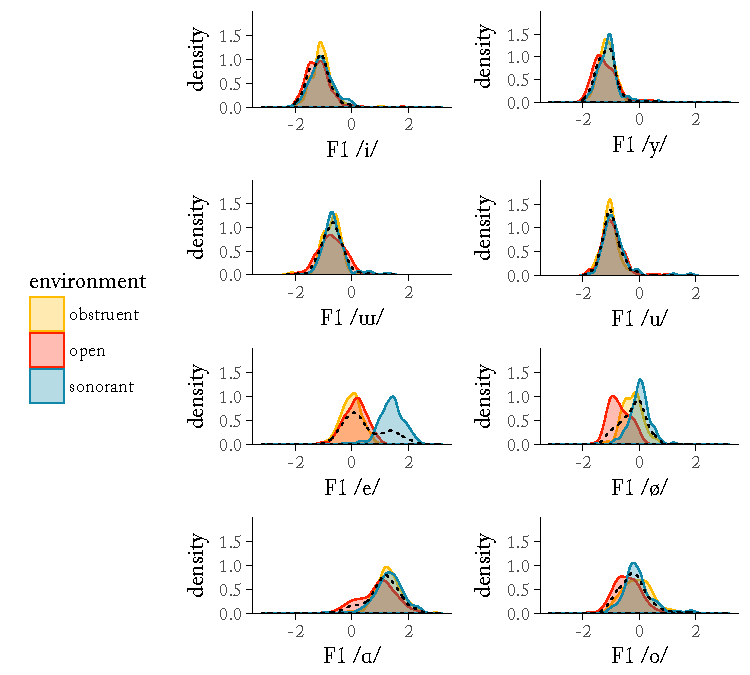
\includegraphics[width=0.49\linewidth]{tr_exploded_density}
    \hfill
  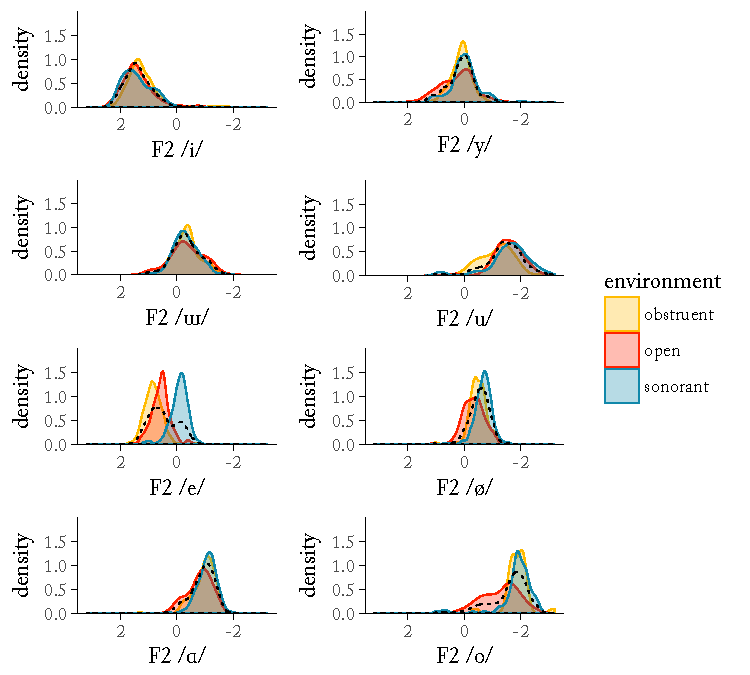
\includegraphics[width=0.49\linewidth]{tr_exploded_density_F2}
  \caption[F1 \& F2 probability density functions, by environment.]{F1 \& F2 probability density functions, by environment. Dotted line: overall PDF from figure \ref{fig:trdensity}.}
  \label{fig:trexploded}
\end{figure}

\subsubsection{The overall picture}

\begin{figure}[H]
  \centering
  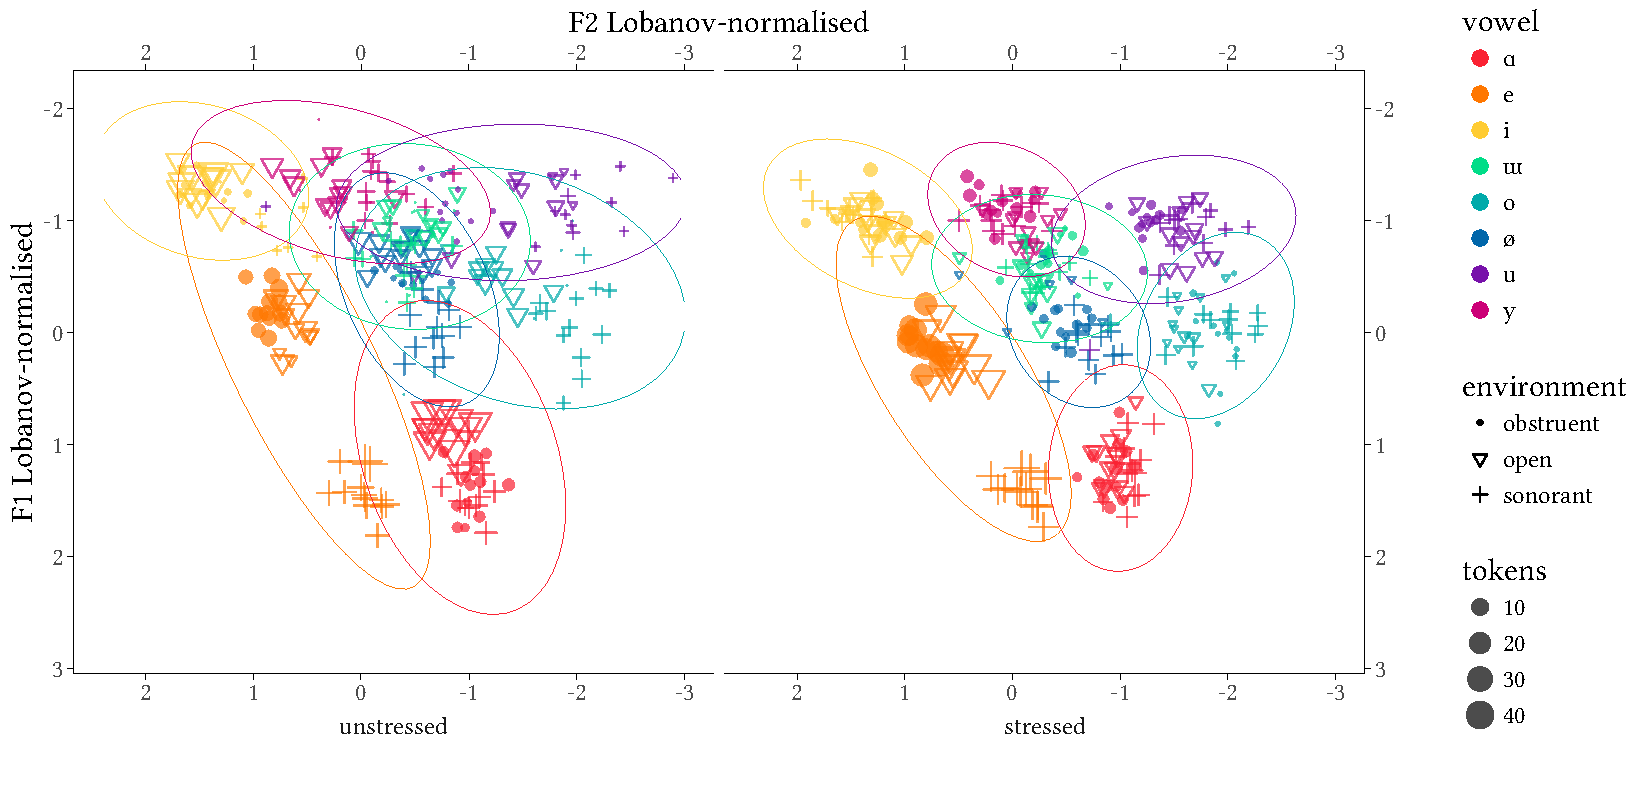
\includegraphics[width=\linewidth]{tr_entire_vowelspace_speaker}
  \caption[F2$\times$F1 space, individual speaker means only.]{F2$\times$F1 space, by vowel category and following environment: each point represents the mean measurement for a single speaker's productions of a particular vowel in the indicated environment; the size of a point denotes the number of tokens represented. 95\% confidence ellipses indicate the overall spread of the \emph{token-by-token} data for a particular vowel.}
  \label{fig:tr_vowelspace_speaker}
\end{figure}

Figure \ref{fig:tr_vowelspace_speaker} shows the Lobanov-normalised F2$\times$F1 space for all 11 \emph{female} speakers, averaged over all tokens across the 8 underlying vowel categories and separated by stress\footnote{For all figures in this paper, `environment' refers to the following segment, and `unstressed' and `stressed' may safely also be read as `non-final' and `final' respectively.}. Each point represents the mean value for a single speaker's productions of a given vowel in a given context, with point size scaled by the number of tokens considered. In \cref{fig:tr_e,fig:tr_ö}, F2$\times$F1 space for /e/ and /\o/ are shown individually, both token-by-token and averaged over the speakers in the sample.

The clear initial generalisation that we reaffirm here is that realisations of /e/ in pre-sonorant contexts diverge strongly and unambiguously from those in other contexts, subject to very little variation; realisations of /ø/ in pre-sonorant contexts also diverge from those in other environments, but the effect appears to be much smaller, and we might claim that there is more variation between speakers. One further striking observation that emerges naturally from \cref{fig:tr_vowelspace_speaker} is the prevalence of strong height effects, presumably coarticulatorily-driven, for open vowels in non-final (that is, unstressed) syllables; the tendency of vowels in unstressed open syllables to be higher (have lower F1) is weak only for /e/.

% \begin{figure}[H]
%   \centering
%   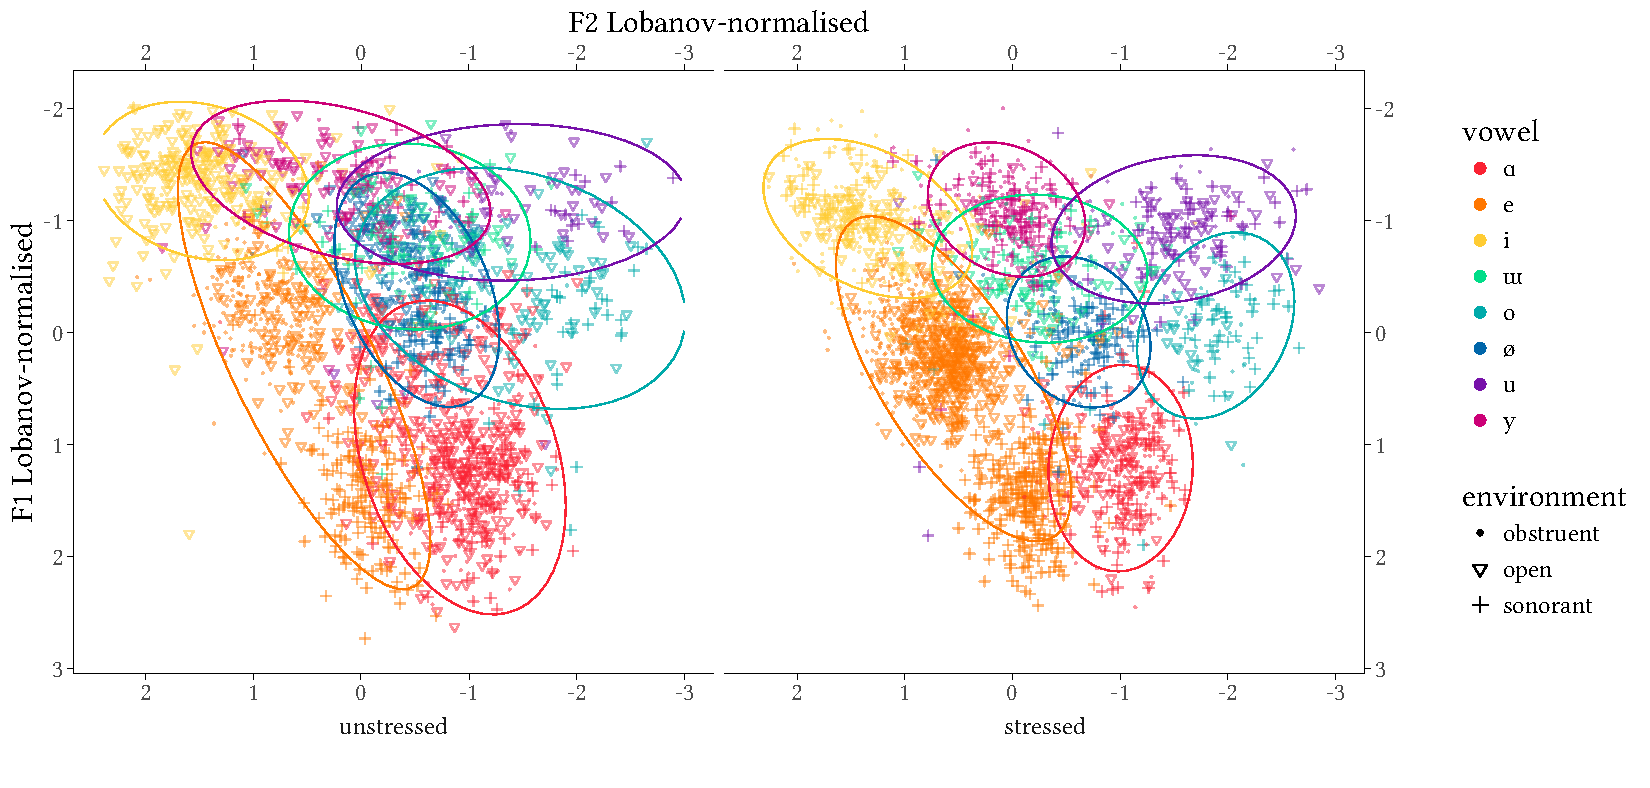
\includegraphics[width=\linewidth]{tr_entire_vowelspace}
%   \caption[F2$\times$F1 space, by vowel category and following environment.]{F2$\times$F1 space, by vowel category and following environment: each point corresponds to a single token, with shape denoting the categorisation of the following coda (obstruent, sonorant, or empty). Ellipses indicate regions of 95\% confidence. }
%   \label{fig:tr_vowelspace}
% \end{figure}

% Run:
%
% f1f2avg()+scale_y_reverse(limits=c(2.5,-1.6),sec.axis = dup_axis(name=''))+scale_x_reverse(position="top",sec.axis = dup_axis(name=''),limits=c(2,-2))+theme(text=element_text(size=15))

\begin{figure}[H]
  \centering
  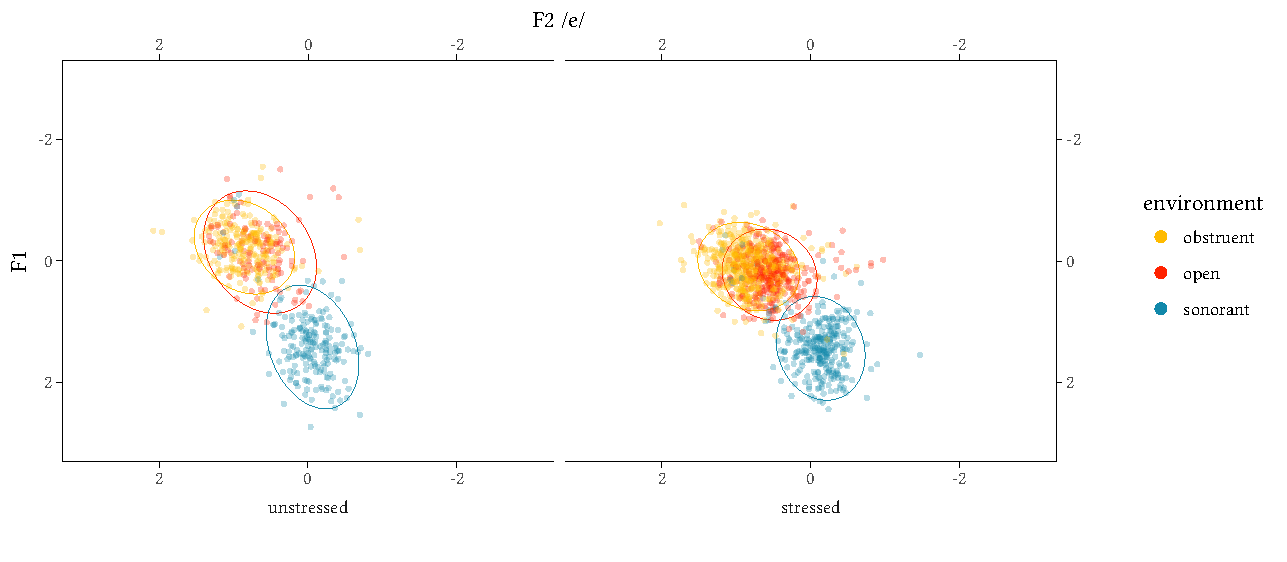
\includegraphics[width=0.8\linewidth]{tr_f1f2_e}
    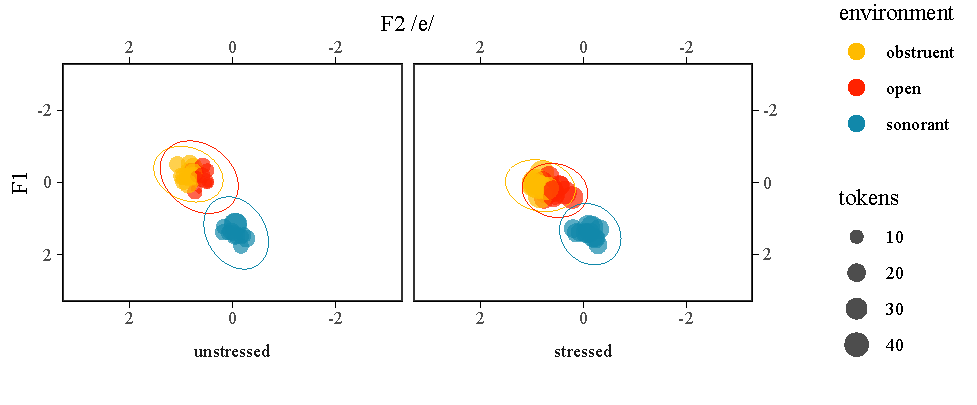
\includegraphics[width=0.8\linewidth]{tr_f1f2_e_speaker}
  \caption[F2$\times$F1 space for /e/ alone by following environment.]{F2$\times$F1 space for /e/, by following environment. Top: each point corresponds to a single token. Bottom: each point corresponds to the mean measurement for a single speaker's productions, with size corresponding to number of tokens. Ellipses indicate regions of 95\% confidence for the token-by-token data in both plots.}
  \label{fig:tr_e}
\end{figure}

\begin{figure}[H]
  \centering
  \includegraphics[width=0.8\linewidth]{tr_f1f2_ö}
    \includegraphics[width=0.8\linewidth]{tr_f1f2_ö_speaker}
  \caption[F2$\times$F1 space for /\o/ alone by following environment.]{F2$\times$F1 space for /\o/, by following environment. Top: each point corresponds to a single token. Bottom: each point corresponds to the mean measurement for a single speaker's productions, with size corresponding to number of tokens. Ellipses indicate regions of 95\% confidence for the token-by-token data in both plots.}
  \label{fig:tr_ö}
\end{figure}


Several preliminary generalisations emerge from \cref{fig:tr_vowelspace_speaker,fig:tr_e,fig:tr_ö}, and from the preceding overview of density. In F2$\times$F1 space, tokens corresponding to pre-sonorant /e/ have essentially no overlap with those corresponding to /e/ in an unclosed or obstruent-closed syllable; the majority of the apparent effect is in F1, with a smaller apparent effect in F2 corresponding roughly to movement along the front diagonal of the vowel space, which we may ascribe entirely to height rather than backness. The relative relationships of the pre-obstruent and open-syllable realisations of /e/ are ambiguous and appear to have some dependence on stress; the overlap is near-complete for unstressed tokens, but stressed pre-obstruent /e/ appears to correspond to slightly increased F2 and slightly reduced F1. The data for /\o/ indicate that some relationship exists between environment and F1; the main contrasts relative to the state of /e/ lie in the lack of distributional discontinuity (although pre-sonorant realisations have the largest F1 values, there is overlap between their range and the ranges for the other environments), and in ordering: for /\o/, realisations in unstressed \emph{open} syllables are consistently the most close (have the lowest value for F1).

Although \cref{fig:tr_e,fig:tr_ö} include speaker averages, they do not indicate the correspondence between individual points and speakers \emph{across categories}. In \cref{fig:tr_speakers_individual}, averaged F1 measurement is visualised, by speaker and environment, for both the mid vowels /e ø/; this is more indicative of the \emph{variation} in the relationship between the three major contexts (and in particular, the relationship between pre-obstruent mean and the open-syllable mean) by individual. Pre-sonorant /e/ is invariant across speakers in its separation from other contexts; the major locus of differences between speakers is the relationship between pre-obstruent /e/ and open-syllable /e/, which varies to the extent of undergoing reversals between individual speakers. Pre-sonorant /ø/ also follows a general speaker-independent trend, but again, individuals vary in the extent to which category separation arises for the other environments. It is reasonable to ask here whether the various loci of individual variation are substantially cross-correlated: do certain /e/-systems correspond to particular /ø/-systems? We revisit this question in \cref{ss:trvariation}, and throughout the discussion that follows, we discuss and model the extent to which the effects that we claim here can be held to be robust and significant.

\begin{figure}[H]
  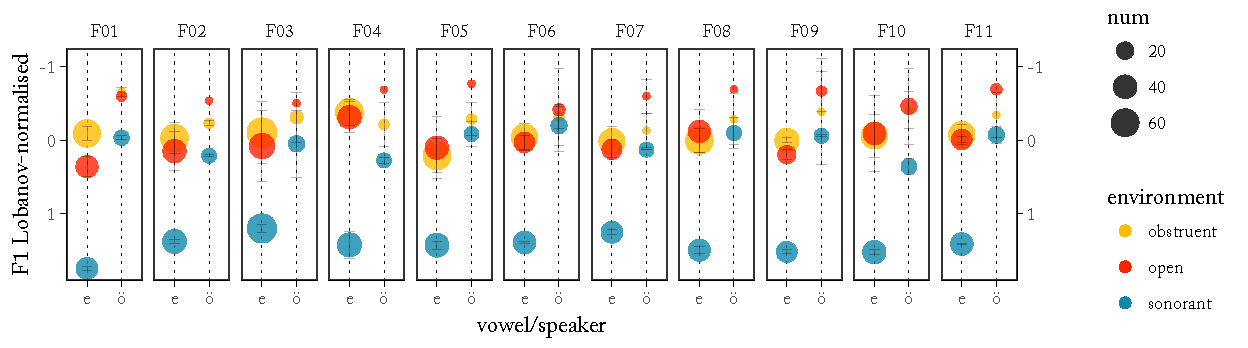
\includegraphics[width=\linewidth]{tr_speakers_vowel.pdf}
  \caption[Normalised F1 by individual speaker, for /e/ and /ø/.]{Normalised F1 by individual speaker, for /e/ and /ø/, averaged over stressed and unstressed contexts. Error bars show one standard deviation.}
  \label{fig:tr_speakers_individual}
\end{figure}

\subsubsection{Significance and effect size}

The previous sub-section offers a broad overview of the environment-mediated patterns visible in the experimental dataset. In the discussion that follows, our aim is to explore some of the available detail; to begin with, we consider the statistical relationship of vowel height to the various possible predictors. In service of this, we fit standard linear mixed-effects models to subsets of the data for /e/ and /\o/ (using R: \texttt{ lme4}, \citealt{lme4}), with F1 as the dependent variable, and the following environment (`obstruent', `sonorant', or `open'), stress (`stressed' or `unstressed'), and their interaction as categorical fixed effects. Potential contributions from individual speaker and lexical item were treated as random effects: models include a random slope of environment and stress by speaker, and of stress\footnote{Not for /ø/, due to the unbalanced nature of the test set; instances of stressed /ø/ were so infrequent that models incorporating a random slope here \emph{do not converge}.} by word. (Another linear mixed-effects model was fitted to investigate the effect of individual sonorant segments (m, n, l, r); for the presentation and discussion of these latter results, see \cref{ss:tr_codas}.) The discussion in following sections, unless otherwise specified, drops the male speakers from the sample.

The choice of mixed-effects models is informed by the possibility of idiosyncracy. There is no a priori reason to expect that individual speakers respond identically to environment or stress; nor is there any reason to expect that all lexical items are treated unexceptionally. The incorporation of \defs{random} effects into a mixed model is then designed to account for this; the inclusion of the \defs{random slope} of stress by speaker, for example, allows the effect of stress (on vowel height) to vary across speakers (different speakers may well implement cues to stress differently, colouring the resultant production).

Summaries of these models are presented below in \cref{tab:tr_lme_e,tab:tr_lme_e_random,tab:tr_lme_ö,tab:tr_lme_ö_random}. These are presented in a standard format\footnote{We're aesthetically indebted here to \cite{Fruehwald2016} for the decision to tabulate density plots for the bootstrapped parameter estimates alongside the model results, and we have done the same throughout.}; as a brief guide, these should be interpreted by the reader as follows. The `base' levels assumed by the model are `obstruent' and `unstressed': the estimate for the mean ($z$-score normalised) F1 in unstressed, pre-obstruent contexts is then given by the intercept, $-0.2074$. In tables corresponding to fixed effects, estimates for further terms predict the difference between these levels and the relevant `base' ones: thus from \cref{tab:tr_lme_e}, the predicted difference between \{open, unstressed\} and \{obstruent, unstressed\} falls in the confidence interval $[-0.1550, 0.1330]$ (indistinguishable from the null, or zero-effect, hypothesis), and the predicted difference between \{open, stressed\} and \{open, unstressed\} falls in the interval $[0.0077, 0.2663]$ (F1 is expected to increase with stress in open syllables).

In tables corresponding to random effects, `variance' and `SD' (standard deviation) are, as in their usual definition, to be interpreted as measures of the spread corresponding to each parameter; that is, in this case, indices of the expected difference in the final value of F1 caused by idiosyncratic speaker or word effects. Correlations represent the extent to which a given fixed effect is invariant for a given random variable. As an example, the perfect correlation between \emph{word} and \emph{stress} in \cref{tab:tr_lme_e_random} really just tells us that given a particular word, `stress' does not vary (that is: /e/ in a particular word is always either stressed or unstressed), and as such is entirely unsurprising. In some situations, a correlation of this type indicates a model that is too complex for the data; however, in this case, there is a theoretical justification for the retention of the stress-word interaction. Even though the value of stress will always remain the same given a particular vowel in a word, there is no reason to expect the \emph{phonetic} effect of that stress on vowel height to be invariant across words; retaining the term in the model allows us to comment on the extent to which the relationship between F1 and stress changes across lexical items.

As an index and as an analytically sound alternative to `$p$-values' in a case in which these are non-meaningful\footnote{Cf. \cite{lme4}: in complex models involving e.g. partially-crossed designs, the null distributions of parameter estimates are not $t$-distributed for finite samples, but computing a $p$-value based on the degrees of freedom for a $t$-distribution (or symmetrically, estimates based on the $F$ statistic) makes such asymptotic assumptions. The well-supported alternative, for the purpose of deciding on significance, is bootstrapping---simulating data from the fitted model, refitting the model, and re-extracting new estimated parameters---from which confidence intervals can be calculated; if the null hypothesis could correspond to points within the confidence interval for a given parameter (i. e. the parameter's effect could be zero), then it cannot be rejected in that context.}, 95\% confidence intervals are given for each fixed term in the model, calculated via semi-parametric bootstrap estimation. Parameters whose value is statistically significant by this measure (that is, non-inclusive of the null) have been marked *. As a guideline, $t$-values greater than 2 should be considered significant.

\begin{table}[H]
  \centering
  \begin{tabular}{lrccr}
    \toprule
    \textsc{Parameter} & \textsc{Estimate} & \textsc{95\% confidence} & \textsc{Bootstrap} & $t$-value\\
    \midrule
    Intercept: obstruent & $-0.21436$ & $[-0.3086, -0.1086]$ & \includegraphics[width=0.1\linewidth]{bootstrap/e_1_intercept} & $-4.267$   \\
    Environment: open & $-0.03109$ & $[-0.1550, 0.1330]$ & 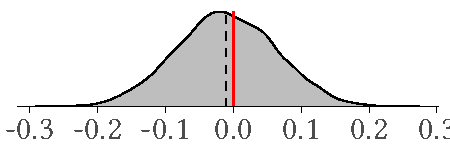
\includegraphics[width=0.1\linewidth]{bootstrap/e_2_open} & $-0.505$ \\
    Environment: sonorant* & $1.61723$ & $[1.510, 1.837]$ & 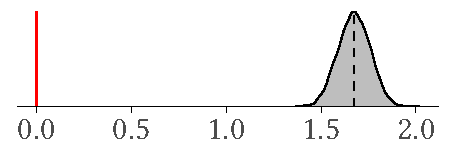
\includegraphics[width=0.1\linewidth]{bootstrap/e_3_son} & $18.716$ \\
    \midrule
    Stress: stressed* & $0.30500$ & $[0.1938, 0.3791]$ & 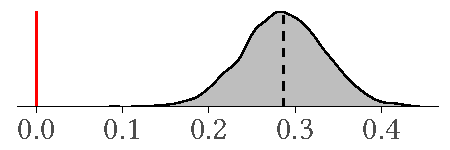
\includegraphics[width=0.1\linewidth]{bootstrap/e_4_stress} & 8.435  \\
    open $\times$ stressed* & $0.15163$& $[0.0077, 0.2663]$ & 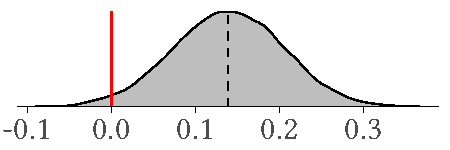
\includegraphics[width=0.1\linewidth]{bootstrap/e_5_stressopen} & 2.464 \\
    sonorant $\times$ stressed* & $-0.37112$ & $[-0.5173, -0.2404]$ & 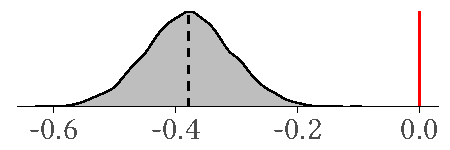
\includegraphics[width=0.1\linewidth]{bootstrap/e_6_stressson} & $-5.205$  \\
    \bottomrule
  \end{tabular}
  \caption[\texttt{\footnotesize F1 $\sim$ environment$\times$stress + (1 + environment + stress|speaker) + (1|word)}, /e/]{Estimated means and derived confidence intervals for fixed effects in the model \texttt{ F1 $\sim$ environment $\times$ stress + (1 + environment + stress|speaker) + (1 + stress|word)} for /e/. 95\% confidence intervals are calculated on 6,000 semi-parametric bootstrap estimates (R: \texttt{ bootMer} from \texttt{ lme4}), for which density plots are shown in the final column. }
  \label{tab:tr_lme_e}
\end{table}

\begin{table}[H]
  \centering\small
  \begin{tabular}{llrrrrr}
    \toprule
    \textsc{Group} & \textsc{} & \textsc{Variance} & \textsc{SD} & \multicolumn{3}{c}{\textsc{Correlation}}\\
    \midrule
    \multirow{2}{*}{\textit{Word}} & Intercept & 0.119126 & 0.34515  \\
                & Stress: stressed & 0.150095 & 0.38742 & $-1.00$  \\
    \midrule
    \multirow{4}{*}{\textit{Speaker}} & Intercept: obstruent & 0.010646 & 0.10318  \\
                & Environment: open                        & 0.021631 & 0.14707   & $-0.18$  \\
                & Environment: sonorant                    & 0.036538 & 0.19115  & $-0.52$ &  0.51    \\
                & Stress: yes                              & 0.007788 & 0.08825  & 0.33    & $-0.23$ &$-0.93$ \\
    \midrule
    \textit{Residual} & & $0.105680$ & $0.32508$ \\
    \bottomrule
  \end{tabular}
  \caption[\texttt{\footnotesize F1 $\sim$ environment$\times$stress + (1 + environment + stress|speaker) + (1|word)}, /e/]{Random effect standard deviations and correlations, model \texttt{ F1 $\sim$ environment $\times$ stress + (1 + environment + stress|speaker) + (1+stress|word)} (\cref{tab:tr_lme_e}), /e/.}
  \label{tab:tr_lme_e_random}
\end{table}

It's evident from \cref{tab:tr_lme_e,tab:tr_lme_ö} that the predicted difference between tokens in sonorant-coda \emph{unstressed} syllables and all other unstressed tokens is large and statistically significant for both /e/ and /\o/, as expected; the interaction with stress is substantial. The presence of (primary) stress reduces F1 in pre-sonorant /e/, but does not remove the large context separation; since, however, this is difficult to clearly adduce from the coefficients presented, as not every possible ordered pair of two-factor interactions is compared by the model\footnote{That is: no coefficient directly compares e. g. \{open, stressed\} and \{sonorant, stressed\}}, \cref{tab:tr_lme_e_stressed} gives the relevant terms and estimates of significance from another mixed-effects model fitted for the \emph{stressed} subset of /e/-tokens alone, with random effects retained as above and the single fixed effect of environment. Modeling predicts no difference between pre-obstruent /e/ and /e/ in open syllables if both are unstressed; \cref{tab:tr_lme_e_stressed} confirms that in stressed contexts, these differ, with F1$_\textsc{obstruent}$ $<$ F1$_\textsc{open}$. We argue that separating out the stressed and unstressed contexts here is not an unprincipled decision; there is a reasonably robust cross-linguistic basis for the claim that these might differ in the phonology, and there \emph{is} an overall significant effect of stress itself on vowel quality. In \cref{sss:coarticulation,ss:trduration}, we argue that there is indeed a larger interaction with stress-conditioned height and duration effects.

\begin{table}[H]
  \centering
  \begin{tabular}{lrccr}
    \toprule
    \textsc{Parameter} & \textsc{Estimate} & \textsc{95\% confidence} & \textsc{Bootstrap} & $t$-value \\
    \midrule
    Intercept: obstruent* & $-0.4835$ & $[-0.7332, -0.2475]$ & \includegraphics[width=0.1\linewidth]{bootstrap/ö_1_intercept} & $-3.410$  \\
    Environment: open* & $-0.3351$ & $[-0.6154, -0.0483]$ & \includegraphics[width=0.1\linewidth]{bootstrap/ö_2_open}& $-2.482$ \\
    Environment: sonorant* & $0.3986$ & $[0.1083, 0.6958]$ & \includegraphics[width=0.1\linewidth]{bootstrap/ö_3_son} & 2.479 \\
    \midrule
    Stress: stressed* & $0.3201$ & $[0.0419, 0.6169]$  & \includegraphics[width=0.1\linewidth]{bootstrap/ö_4_stress} & 2.140  \\
    open $\times$ stressed\footnotemark & $0.2117$ & $[-0.3531, 0.7609]$ & \includegraphics[width=0.1\linewidth]{bootstrap/ö_5_stressopen} & 0.822 \\
    sonorant $\times$ stressed & $-0.1411$ & $[-0.4973, 0.2118]$ & \includegraphics[width=0.1\linewidth]{bootstrap/ö_6_stressson} & $-0.872$  \\
    \bottomrule
  \end{tabular}
  \caption[\texttt{\footnotesize F1 $\sim$ environment$\times$stress + (1 + environment + stress|speaker) + (1|word)}, /\o/]{Estimated means and derived confidence intervals for fixed effects in the model \texttt{F1 $\sim$ environment $\times$ stress + (1 + environment + stress|speaker) + (1|word)} for /\o/. 95\% confidence intervals are calculated on 6,000 semi-parametric bootstrap estimates, for which density plots are shown in the final column. }
  \label{tab:tr_lme_ö}
\end{table}
\footnotetext{Recall that only four data points went into this estimate.}

\begin{table}[H]
  \centering\small
  \begin{tabular}{llrrrrr}
    \toprule
    \textsc{Group} & \textsc{} & \textsc{Variance} & \textsc{SD} & \multicolumn{3}{c}{\textsc{Correlation}}\\
    \midrule
    \multirow{1}{*}{\textit{Word}} & Intercept & 0.04007 & 0.2002 & & &  \\
    \midrule
    \multirow{4}{*}{\textit{Speaker}} & Intercept: obstruent & 0.01806 &  0.1344  \\
                & Environment: open                        & 0.02618 & 0.1618  & $-0.95$   \\
                & Environment: sonorant                    &0.02657 &  0.1630 & $ -0.16$ & 0.46    \\
                & Stress: yes                              & 0.02133 & 0.1461  & $-0.49$ & 0.29 & $-0.38$ \\
    \midrule
    \textit{Residual} & & 0.07373 & 0.2715 \\
    \bottomrule
  \end{tabular}
  \caption[\texttt{\footnotesize F1 $\sim$ environment$\times$stress + (1 + environment + stress|speaker) + (1|word)}, /e/]{Random effect standard deviations and correlations, model \texttt{ F1 $\sim$ environment $\times$ stress + (1 + environment + stress|speaker) + (1|word)} (\cref{tab:tr_lme_ö}), /ø/.}
  \label{tab:tr_lme_ö_random}
\end{table}

\begin{table}[H]
  \centering
  \begin{tabular}{lrccr}
    \toprule
    \textsc{Parameter} & \textsc{Estimate} & \textsc{95\% confidence} & \textsc{Bootstrap} & $t$-value\\
    \midrule
    Intercept: obstruent & $0.08364$ & $[-0.0154, 0.1801]$ & 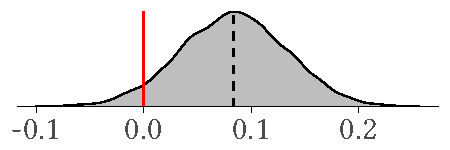
\includegraphics[width=0.1\linewidth]{bootstrap/es_1_intercept} & 1.663 \\
    Environment: open* & $0.11841$ & $[0.0093, 0.2248]$ & 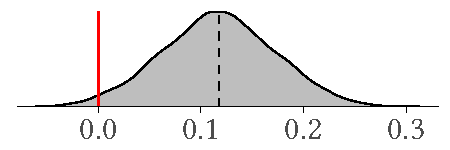
\includegraphics[width=0.1\linewidth]{bootstrap/es_2_open} & 2.147\\
    Environment: sonorant* & $1.32594$ & $[1.183, 1.472]$ & 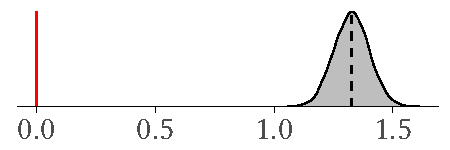
\includegraphics[width=0.1\linewidth]{bootstrap/es_3_son} & 17.674\\
    \bottomrule
  \end{tabular}
  \caption[\texttt{\footnotesize F1 $\sim$ environment + (1 + environment|speaker) + (1|word)}, /e/]{Estimated means and derived confidence intervals for fixed effects in the model \texttt{ F1 $\sim$ environment + (1 + environment|speaker) + (1|word)} for \emph{stressed} /e/ only. 95\% confidence intervals are calculated on 6,000 semi-parametric bootstrap estimates (R: \texttt{ bootMer} from \texttt{ lme4}), for which density plots are shown in the final column. }
  \label{tab:tr_lme_e_stressed}
\end{table}

\begin{table}[H]
  \centering\small
  \begin{tabular}{llrrrrr}
    \toprule
    \textsc{Group} & \textsc{} & \textsc{Variance} & \textsc{SD} & \multicolumn{3}{c}{\textsc{Correlation}}\\
    \midrule
    \multirow{1}{*}{\textit{Word}} & Intercept & 0.02551 & 0.1597 & & &  \\
    \midrule
    \multirow{4}{*}{\textit{Speaker}} & Intercept: obstruent & 0.02285 &  0.1512  \\
                & Environment: open                        & 0.01548 & 0.1244  & $-0.20$   \\
                & Environment: sonorant                    &0.04737 &  0.2176 & $ -0.83$ & 0.40    \\
    \midrule
    \textit{Residual} & & 0.09305 & 0.3050 \\
    \bottomrule
  \end{tabular}
  \caption[\texttt{\footnotesize F1 $\sim$ environment$\times$stress + (1 + environment + stress|speaker) + (1|word)}, /e/]{Random effect standard deviations and correlations, model \texttt{ F1 $\sim$ environment $\times$ stress + (1 + environment + stress|speaker) + (1|word)} (\cref{tab:tr_lme_e_stressed}), stressed /e/.}
  \label{tab:tr_lme_e_stressed_random}
\end{table}

There is a real, persistent, and statistically-significant effect of environment on the first formant for both /e/ and /ø/. Our inability to diagnose a statistically meaningful split between pre-obstruent and open-syllable /e/ we take as \emph{inconclusive} rather than definitively \emph{negative}, and revisit the problem in the discussion of individual variation in \cref{ss:trvariation}. Effects are given in $z$-score measures throughout, which scale the whole dataset to a normal distribution with mean 0 and standard deviation 1; in order to grasp the meaning of the expected values given here, each linear-model estimate can then be understood to correspond to a number of standard deviations across the whole vowel space. This is not small; as an index of comparison, one standard deviation in F1 across the {raw} (non-normalised) dataset is 164 Hz. If we ask how this compares to the threshold for \emph{perceptual} significance, one index of a possible answer is the range of typical values guaranteeing reliable perceptibility in experimentation. Cross-linguistic work on formant-frequency discrimination \citep{KewleyPort1994,KewleyPort2005} suggests that the baseline $\Delta$F1 required for reliable perceptual discrimination is in the region of 20Hz, so effects greater than around $z$ $\pm 0.12$ over our whole dataset are plausibly perceptually meaningful and interesting.

\subsection{Triggering segments}\label{ss:tr_codas}\todo{Keep all this information, but reorganise — data first, then make the point that it's rhotic triggered, rhotic loses 'control' relatively quickly, and rate of change / degree of change is not proportional to phonetic precursor-ness}

In \cref{sss:tr_son_effects}, we considered the extent to which the individual sonorants constitute robust \defs{phonetic precursors} to vowel lowering. The answer is not entirely conclusive; but the strength of the precursor in each environment does not seem to be constant, and the cross-linguistic evidence is variable. Further phonetic discussion of the case of the Turkish lateral appears in \cref{sss:lateral} below; we argue therein that the lateral in Turkish does not represent a strong acoustic-articulatory trigger for vowel lowering.

If it is really the case that different coda sonorants constitute different sizes of trigger, then we might well expect a difference in within-context realisations of pre-sonorant /e ø/, further conditioned by the individual coda segment. If this difference is visible in the data, how should it be understood? To recapitulate a little of the discussion in \cref{s:tr_classtype} with a visual example, models of sound change as \defs{hypocorrecting} change \citep{Ohala1981} should predict that precursors of different strengths \emph{induce effects of different sizes} and thus cause change to take place at different rates across the different coda contexts; as \citet{Fruehwald2016}, hypocorrective changes proceed proportionally to the sizes of their precursors. Assume a hypothetical parameter $p$, which varies over time in several different contexts; at each time step, $p$ is incremented by an amount corresponding to a contextual bias favouring change. For contexts corresponding to biases of 0.1, 0.25, and 0.5 respectively, the parameter's evolution over time appears in \cref{fig:tr_hypo_example} (after \citealt[378]{Fruehwald2016}); after a few steps, values across contexts are further apart than they were initially.

\begin{figure}[H]
  \centering
  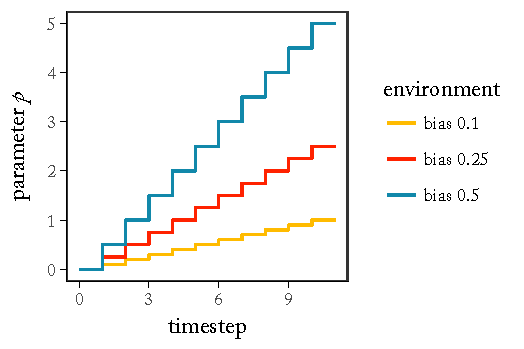
\includegraphics[width=0.45\linewidth]{tr_hypocorrecting}
  \caption[A rough illustration of hypocorrection.]{A prototype of a \emph{purely hypocorrecting} change: different biases cause unequal incrementation and different end realisations of phonetically-controlled parameter $p$. Conditions: $p$ starts at 0, and is incremented by the value of the bias at each time step. }
  \label{fig:tr_hypo_example}
\end{figure}

There are then multiple possible interpretations if we find a real statistical effect differentiating one pre-sonorant context from another. If the pathway of change was the one schematised in \cref{fig:tr_hypo_example}, then a visible difference across coda sonorants represents the end-product (or the intermediate point) of a hypocorrecting change: if the mechanism of phonologisation \emph{remains} strictly hypocorrecting throughout, then we expect the effect of the initial difference in bias strength to be linearly multiplied over time. The alternate hypothesis is that the incrementation of phonological change is not strictly proportional to the strength of contextual phonetic biases; any visible difference across coda sonorants should be taken to represent \emph{the original} triggering bias, but not the incrementation and compounding of that bias. If the fictional parameter in \cref{fig:tr_hypo_example} is subject to an \emph{initial} `phonetic' bias differentiating its values across contexts, but then undergoes a fixed increment at each time step, we arrive at the situation in \cref{fig:tr_nonhypo_example}.

\begin{figure}[H]
  \centering
  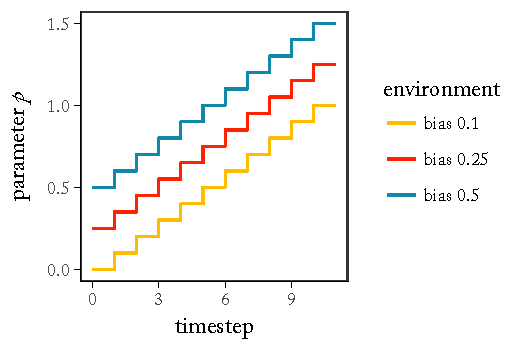
\includegraphics[width=0.45\linewidth]{tr_linear}
  \caption[A rough illustration of constant-slope change.]{Change with a non-additive bias; we still see different end realisations of the phonetically-controlled parameter $p$, but the size of the contextual effect now remains constant. Initial conditions: $p$ is 0.1, 0.25, 0.5 in the appropriate contexts, and is incremented by 0.1 at each time-step.}
  \label{fig:tr_nonhypo_example}
\end{figure}

Within the set of sonorant triggers---the nasals, the lateral, and the rhotic---do further effects exist, either globally or subject to interspeaker variation? One possibility is that the final state of pre-sonorant /e/ and /\o/ realisations is further differentiated by coda segment; if this differentiation exists and corresponds to the `strength' of the phonetic precursor provided by a given coda segment, this would fall in line with predictions about the end state of a hypocorrective, phonetically-motivated and bias-driven change (cf. \cref{s:tr_introduction}), but the absence of either of these properties might point to a different pathway. In the case under consideration, one way to test which of these interpretations is more meaningful is to consider those tokens for which lowering is blocked by the placement of the syllable boundary. Recall (\cref{ss:trcase}) that resyllabification under affixation blocks lowering, as in [gi.zæm] `mystery' but /gizem-i/ [gi.ze.mi] `mystery-\textsc{\footnotesize dat}'; in open syllables preceding an onset sonorant, we do not predict the existence of any systematic, grammatically-controlled lowering. If it is the case that there exists an effect differentiating tokens of /e/ in open syllables followed by \emph{onset} /r/ from other tokens of /e/ in non-final open syllables, we should find it reasonable to conclude that there is a phonetic effect of post-vocalic rhotics. If it is also the case that this effect is `similar' in size to any effect distinguishing tokens preceding \emph{coda} rhotics from those preceding other coda sonorants, then we suggest that the phonologisation of /e/-lowering has not in itself left behind the phonetic trace that pure-hypocorrecting accounts predict.

Consider the F2$\times$F1 scatterplots given in \cref{fig:tr_e_codas,fig:tr_ö_codas}; these represent a subset of the data corresponding to all tokens followed by coda /r/, /l/, /m/, /n/ only. Each point represents a single pre-sonorant token of /e/ and /\o/ respectively, with 95\% confidence ellipses indicating the spread of realisations. Inspection suggests that there is no substantial discontinuity and certainly no further categorical allophony; there is a slight predominance of pre-rhotic /e/ tokens at higher F1 values (lower, more open realisations).

Examining the F2$\times$F1 landscape after averaging and weighting by speaker (\cref{fig:tr_e_speaker}), however, suggests that the majority of this pre-rhotic effect can be attributed to productions from two speakers, F01 (Istanbul, b. 1997) and F04 (Izmir, b. 1988). F01 shows a generally higher F1 across contexts than other speakers, but all cross-context variation is well within confidence intervals and cannot be attributed to a `real' effect. The separation between pre-rhotic tokens and other pre-sonorant tokens for F04 appears genuinely significant, and may represent an individual idiosyncracy in production. In the following \cref{sss:trcodamodel}, statistical models are presented that account for interspeaker variation.

\begin{figure}[H]
  \centering
  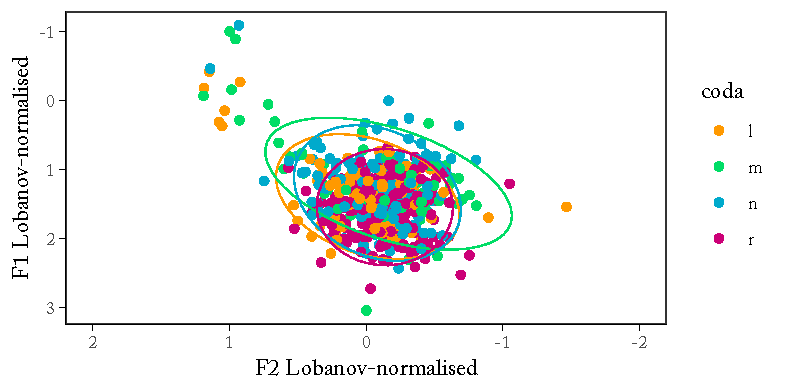
\includegraphics[width=0.75\linewidth]{tr_son_e}
  \caption[F2$\times$F1 space for pre-sonorant /e/, by individual coda segment.]{F2$\times$F1 space for pre-sonorant /e/, by individual coda segment. Each point corresponds to one vowel produced by a single speaker.}
  \label{fig:tr_e_codas}
\end{figure}

\begin{figure}[H]
  \centering
  \includegraphics[width=0.75\linewidth]{tr_son_ö}
  \caption[F2$\times$F1 space for pre-sonorant /\o/, by individual coda segment.]{F2$\times$F1 space for pre-sonorant /\o/, by individual coda segment. Each point corresponds to one vowel produced by a single speaker.}
  \label{fig:tr_ö_codas}
\end{figure}

\begin{figure}[H]
  \centering
  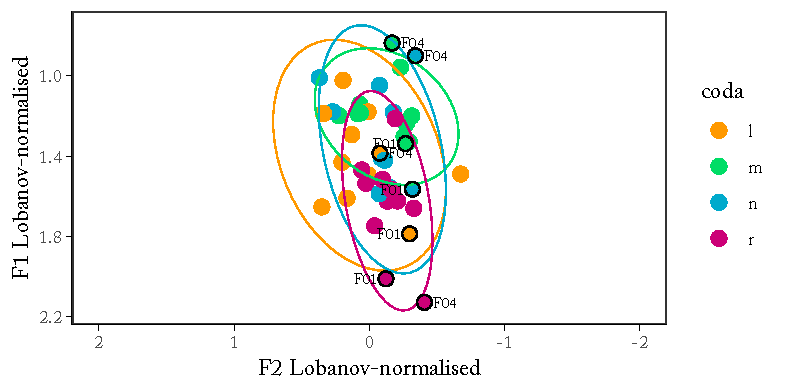
\includegraphics[width=0.75\linewidth]{tr_son_e_speaker}
  \caption[F2$\times$F1 space for pre-sonorant /e/, averaged by speaker and coda.]{F2$\times$F1 space for pre-sonorant /e/, by individual coda segment. Each point corresponds to the \textit{mean} of all corresponding tokens for a single speaker. Speakers F01 and F04, both of whom show particularly high F1 values in pre-rhotic contexts, are highlighted.}
  \label{fig:tr_e_speaker}
\end{figure}

Consider further the scatterplot given in \cref{fig:tr_e_open_codas}, representing all tokens of /e/ in \emph{unstressed open syllables} immediately followed by an onset sonorant across the syllable boundary. Although the number of tokens is not large, there is some evidence to suggest that there is a meaningful effect of the rhotic on a vowel that precedes it \emph{across} a syllable boundary. Vowels in open syllables are very susceptible to other height effects (\cref{sss:coarticulation,ss:trduration}); with this said, even though the conditions for raising effects are met in many of the pre-sonorant tokens here, their distribution is even across the set of lexical items that appears in \cref{fig:tr_e_open_codas}, which appears below in \cref{tab:tr_e_open_codas}. Contexts in which the \emph{raising} of \cref{sss:coarticulation} might be expected to apply are indicated by shaded cells.

\begin{table}[H]
\centering
\begin{tabular}{cccc}
  \toprule
r & l & n & m\\
\midrule
be.ra.ber      & ka.le.ler      & \yes fe.ni & \yes er.de.mi \\
\yes def.te.ri & \yes ge.lir    & men.ge.ne  & el.le.mek \\
sek.re.ter     & ker.ten.ke.le  & ge.nel     & te.mel \\
\bottomrule
\end{tabular}
\caption{Items in the test set containing open syllable /e/ followed by a sonorant onset.}
\label{tab:tr_e_open_codas}
\end{table}

\begin{figure}[H]
  \centering
  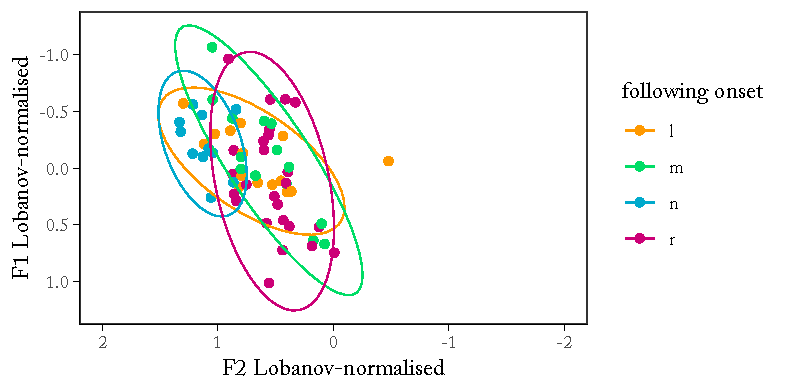
\includegraphics[width=0.75\linewidth]{tr_e_open_coda}
  \caption[F2$\times$F1 space for /e/ in open syllables preceding sonorant onsets.]{F2$\times$F1 space for /e/ in \textit{open syllables}, by the content of the immediately following syllable onset. Each point corresponds to one vowel produced by a single speaker.}
  \label{fig:tr_e_open_codas}
\end{figure}

\subsubsection{Modeling}\label{sss:trcodamodel}

Do individual [sonorant] segments in fact trigger different degrees of /e/-lowering or /\o/-lowering, despite the unclear state of such effects on visual inspection? A more reliable route to an evaluation of the significance of particular coda environments is modeling: as before, and for similar reasons, we fit two further mixed-effects models---for /e/ and /\o/ respectively---to a subset of the data consisting solely of those tokens with a coda sonorant in the right-hand environment, with F1 as dependent variable, coda (m, n, l, r) and stress (`stressed' or `unstressed') as categorical fixed effects. Summaries of these results are presented in \cref{tab:tr_lme_e_coda,tab:tr_lme_ö_coda}, including confidence intervals calculated via semi-parametric bootstrap estimation; the base levels assumed by the model are `coda /l/' and `unstressed'.

The model in \cref{tab:tr_lme_e_coda} does not support a claim that a significant difference exists between \emph{pre-lateral} /e/ and \emph{pre-rhotic} /e/. Realisations preceding \emph{nasals} are generally higher (lower values of F1); what cannot be diagnosed from this analysis is whether this represents a systematic property of the phonologically-conditioned environments, or a `top-level' effect of nasalisation in pre-nasal vowels (driven by the presence of nasal anti-formants).

\begin{table}[H]
  \centering
  \begin{tabular}{lrccc}
    \toprule
    \textsc{Parameter} & \textsc{Estimate} & \textsc{95\% confidence} & \textsc{Bootstrap}\\
    \midrule
    Intercept: coda /l/ & $1.47751$ & $[1.230, 1.726]$ & \includegraphics[width=0.1\linewidth]{bootstrap/son/e_1_intercept}  \\
    Coda: /m/* & $-0.44463$ & $[-0.7648, -0.1452]$ & 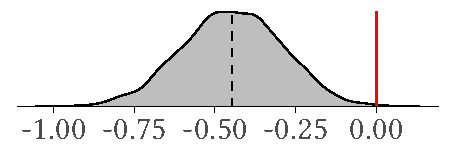
\includegraphics[width=0.1\linewidth]{bootstrap/son/e_2_m} \\
    Coda: /n/* & $-0.33914$ & $[-0.6501, -0.0239]$ & 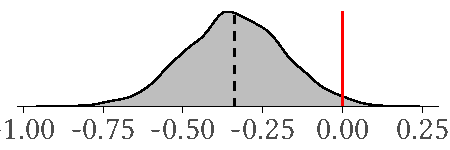
\includegraphics[width=0.1\linewidth]{bootstrap/son/e_3_n} \\
    Coda: /r/ & $0.08575$ & $[-0.1924, 0.3616]$ & 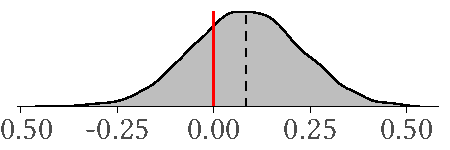
\includegraphics[width=0.1\linewidth]{bootstrap/son/e_4_r}   \\
    \midrule
    Stress: stressed* & $-0.14399$ & $[-0.4413, 0.1428]$ & 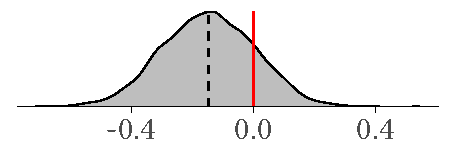
\includegraphics[width=0.1\linewidth]{bootstrap/son/e_5_stress}   \\
    coda /m/ $\times$ stressed & $0.21697$ & $[-0.2289, 0.6633]$ & 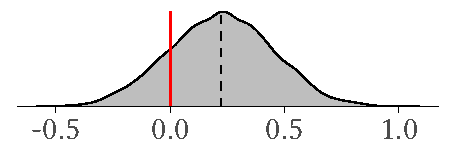
\includegraphics[width=0.1\linewidth]{bootstrap/son/e_6_stressm} \\
    coda /n/ $\times$ stressed & $0.37876$ & $[-0.0244, 0.7911]$ & 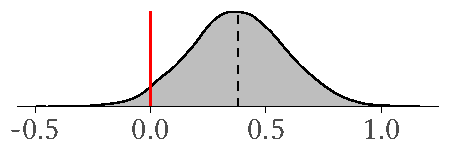
\includegraphics[width=0.1\linewidth]{bootstrap/son/e_7_stressn} \\
    coda /r/ $\times$ stressed & $0.08133$ & $[-0.2982, 0.4731]$ & 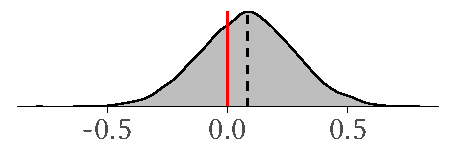
\includegraphics[width=0.1\linewidth]{bootstrap/son/e_8_stressr}   \\
    \bottomrule
  \end{tabular}
  \caption[\texttt{\footnotesize F1 $\sim$ coda $\times$ stress + (1 + coda + stress|speaker) + (1|word)}, /e/]{Estimated means and derived confidence intervals for fixed effects in the model \texttt{ F1 $\sim$ coda $\times$ stress + (1 + coda + stress|speaker) + (1|word)} for /e/. 95\% confidence intervals are calculated on 6,000 semi-parametric bootstrap estimates (R: \texttt{ bootMer} from \texttt{ lme4}), for which density plots are shown in the final column. }
  \label{tab:tr_lme_e_coda}
\end{table}

\begin{table}[H]
  \centering
  \begin{tabular}{lrccc}
    \toprule
    \textsc{Parameter} & \textsc{Estimate} & \textsc{95\% confidence} & \textsc{Bootstrap}\\
    \midrule
    Intercept: coda /l/ & $-0.21494$ & $[-0.4132, -0.0175]$ & \includegraphics[width=0.1\linewidth]{bootstrap/son/ö_1_intercept}  \\
    Coda: /m/ & $0.22929$ & $[-0.0273, 0.4198]$ & \includegraphics[width=0.1\linewidth]{bootstrap/son/ö_2_m} \\
    Coda: /n/ & $0.13411$ & $[-0.0567, 0.3241]$ & \includegraphics[width=0.1\linewidth]{bootstrap/son/ö_3_n} \\
    Coda: /r/* & $0.20231$ & $[0.0249, 0.3791]$ & \includegraphics[width=0.1\linewidth]{bootstrap/son/ö_4_r}   \\
    \midrule
    Stress: stressed & $0.20982$ & $[-0.0164, 0.4321]$ & \includegraphics[width=0.1\linewidth]{bootstrap/son/ö_5_stress}   \\
    coda /m/ $\times$ stressed & \multicolumn{2}{c}{\emph{no tokens, dropped from model}} & \includegraphics[width=0.1\linewidth]{bootstrap/son/ö_6_stressm} \\
    coda /n/ $\times$ stressed & $0.14977$ & $[-0.1268, 0.4321]$ & \includegraphics[width=0.1\linewidth]{bootstrap/son/ö_7_stressn} \\
    coda /r/ $\times$ stressed & $-0.13339$ & $[-0.3727, 0.1141]$ & \includegraphics[width=0.1\linewidth]{bootstrap/son/ö_8_stressr}   \\
    \bottomrule
  \end{tabular}
  \caption[\texttt{\footnotesize F1 $\sim$ coda $\times$ stress + (1 + coda + stress|speaker) + (1|word)}, /\o/]{Estimated means and derived confidence intervals for fixed effects in the model \texttt{ F1 $\sim$ coda $\times$ stress + (1 + coda + stress|speaker) + (1|word)} for /\o/. 95\% confidence intervals are calculated on 6,000 semi-parametric bootstrap estimates (R: \texttt{ bootMer} from \texttt{ lme4}), for which density plots are shown in the final column. }
  \label{tab:tr_lme_ö_coda}
\end{table}

\subsubsection{The lateral}\label{sss:lateral}

In \cref{ss:coda_effects}, we discussed possible motivations, phonetic and structural, for anticipatory F1-lowering, with the note that the status of the lateral would be addressed in greater depth in the following sections. What we are interested in here is whether or not the lateral itself constitutes an independently-motivated trigger for a vowel height effect: recall the discussion in \cref{s:tr_introduction,s:tr_classtype}, in which it was proposed that the analysis of the `naturalness' of active classes in phonological change should take into account the individual likelihood that each segment in that class constitutes a plausible phonetic precursor to the change in question, rather than the overall structure of the class alone.

I reference in \cref{sss:trphonology} the descriptive claim that the Turkish /l/ has an allophonic distribution conditioned by the backness of the surrounding vowel. The expected status of the lateral as a phonetic precursor to height effects then has a necessary dependence on its status as plain, velarised, or palatalised; these impressionistic categories correspond to a significant degree of acoustic variation (\citealt{Proctor2009} for an overview). Acoustic studies of various laterals suggest a correspondence between the first two formants and the degree of `darkness', with a larger F2$\times$F1 difference corresponding to a `lighter' (and thus further fronted) [l] \citep{Sproat1993,Turton2014,Carter2002,Recasens2005}. The locus of this difference is largely in F2 variation, with F1 relatively invariant throughout even in dynamic analysis \citep{Strycharczuk2016}, but due to the non-independence of F1 and F2 a correspondence is expected between backing (decrease) in F2 and openness (increase) in F1; \cite{Sproat1993,Carter2007} give increased F1 as a secondary correlate of /l/-darkness,  If anticipatory coarticulation with a lateral affects the quality of the vowel immediately prior, we may then hypothesise that the major effect of a \emph{velarised} lateral on a front vowel, corresponding in gestural terms to predorsum lowering and postdorsum retraction \citep{Recasens2012}, would be reflected in a F2 decrease from the V target towards the lower /l/-target. It is less clear that a fronted lateral should cause an increase in F1 as an anticipatory coarticulatory effect, since the predicted transition into such a lateral from a mid vowel involves a drop in F1 and a sharp increase in F2; indeed, the tongue-tip gesture corresponding to alveolarity corresponds rather to predicted raising, and thus F1-decrease. \cite{Recasens2014} gives /e/-lowering to [a] post-palatal lateral in Catalan as a possible progressive dissimilatory process in a very small handful of cases, but gives pre-lateral raising as far more frequent. \todo{Diskin et al lowering in Melbourne — see if anything relevant to cite}

The remarks in this section constitute a very preliminary study of the acoustic properties of the Turkish lateral; the intent is not at all to provide a full study, but to characterise in broad strokes the expected nature of the transition in /el/: can /e/-lowering in /el/ admit a simple coarticulatory explanation? In order to test this, all instances of /l/ were extracted from the production data collected in this study, for measurement. Across 11 (female) speakers, this yielded 627 tokens for analysis; of these, 53 were discarded due to regressive manner assimilations (to coronals s, z, n) or due to phrase-final devoicing and frication leading to unreliable formant measurements. For the remaining 574 datapoints, F1 and F2 were measured at the midpoint, to give a rough indicator of the `frontness' of the lateral. A summary visualisation appears in \cref{fig:trlateral}; tokens were coded `front', `back', and `disharmonic' by adjacent vowel (respectively: exclusively i, y, e, \o; exclusively ɯ, u, a, o; one vowel from both sets).

\begin{figure}[H]
  \centering
  \includegraphics[width=\linewidth]{tr_laterals}
  \caption[F2$\times$F1 distribution for the lateral /l/ by vocalic environment.]{F2$\times$F1 space for the lateral /l/, measured at midpoint, by vocalic environment: `disharmonic' tokens are adjacent in the string to both a front vowel (i, e $\sim$ æ, y, ø $\sim$ œ) and a back vowel (ɯ, u, o, ɑ), within a single syllable or across the syllable boundary.}
  \label{fig:trlateral}
\end{figure}

\begin{figure}[H]
  \centering
  \includegraphics[width=\linewidth]{tr_laterals_position}
  \caption[F2$\times$F1 distribution for fronted /l/ by syllabic position.]{F2$\times$F1 space for \textit{fronted} tokens of lateral /l/, measured at midpoint, by position.}
  \label{fig:trlateral_pos}
\end{figure}

The distribution of the Turkish laterals in F2$\times$F1 space thus appears discontinuous and categorical, conditioned by the adjacent vowels and with no particular dependence on syllabic position. Without exception, the laterals adjacent to (either preceded by or preceding) front vowels have significantly raised F2, including those occupying codas immediately following phonologically lowered /e/ [\ae]. Other plausible predictors (vowel quality, stress) had no statistically meaningful effect.

Why are the realisational details of the Turkish coda lateral interesting to us? In a language like English, in which the distribution of the plain lateral and the heavily velarised lateral is strictly conditioned by position in the syllable, the velarised coda lateral becomes a natural and well-motivated phonetic trigger for vocalic effects. In any of the contexts in which we are interested in the Turkish lateral, however, \emph{no such trigger exists}.

\subsection{Duration}\label{ss:trduration}

One possible origin for the vowel-lowering alternations that we see is in coda-conditioned loss or gain of duration, as in the analyses of vowel quality effects that we cover in \cref{sss:csvl}. If this is the case, then we might expect some systematic pattern to appear in the sample; both in the duration-F1 correlation, and in the predicted duration for each phonologically-active set of environments (pre-obstruent; pre-sonorant; open).

\subsubsection{/i/-triggered height effects}\label{sss:coarticulation}

Recall from \cref{tab:tr_lme_e,tab:tr_lme_e_stressed} that there were statistically-significant estimates distinguishing /e/-realisations in \emph{stressed} and \emph{unstressed} open syllables, and in \emph{stressed} syllables for each of the three environment types, but that we could not reject the zero-difference hypothesis for `obstruent' and `open' in unstressed syllables. In terms of our estimated parameters, this is as follows: F1$_\textsc{obstruent}$ $\sim$ F1$_\textsc{open}$ $<$ F1$_\textsc{sonorant}$ in unstressed syllables, but F1$_\textsc{obstruent}$ $<$ F1$_\textsc{open}$ $<$ F1$_\textsc{sonorant}$ in unstressed syllables. Both cases for /e/ are distinct from the case for unstressed /o/, for which F1$_\textsc{open}$ $<$ F1$_\textsc{obstruent}$ $<$ F1$_\textsc{sonorant}$. One possibility is that the state of unstressed /e/ is in fact a \emph{superposition} of an /o/-like case (open $<$ obstruent $<$ sonorant) and a stressed-/e/-like case (obstruent $<$ open $<$ sonorant).

\begin{figure}[H]
  \centering
  \includegraphics[width=0.8\linewidth]{tr_heightharmony}
  \caption[F2$\times$F1 space for /e/ in unstressed open syllables.]{F2$\times$F1 space for /e/, with the high vowels /i/ and /y/. Ellipse: 95\% confidence region for tokens of \textbf{/i/}. One point corresponds to the \emph{mean} across all tokens of a single word.}
  \label{fig:trheightharmony}
\end{figure}

Consider the F2$\times$F1 space depicted in \cref{fig:trheightharmony} above. All items of the form /(C)e.Ci/ are highlighted and transcribed; /e/-realisations in these contexts fall within the bounds of tolerance for the high vowel /i/, and skew the overall F1-distribution for /e/ in open syllables. This then suggests that there is something special about the unstressed open syllables; we refrain from answering the resultant questions now, but the problem will recur in \cref{ss:trduration,ss:trvariation}.

\subsubsection{The duration-height connection}

In \cref{sss:csvl}, we devoted some attention to the relationship between duration and vowel quality; what we did not address in full was the state of the debate as to whether this relationship has a purely mechanical etiology, or instead arises from the variable phonologisation of durational targets. The mechanical explanation, rooted solely in facts of articulation and low-level phonetics; makes several fundamentally testable predictions. If low vowels are longer due to the length of the jaw-opening gesture \citep{Lehiste1970}, then the `extra' length must be particularly visible in the onset and offset formant movements towards the low vowel \citep{Lisker1974}; if instead the steady-state is the locus of increased duration, this argues for a phonological explanation. If durational effects are purely mechanical, then they should remain constant across speech rates; \cite{Sole2010} find that this is indeed the case in Japanese, but is not the case in Catalan or English, and argue therefore that the correlation between F1 and duration is phonologically-controlled in the latter languages but phonetically-controlled in the former. Two further predictions of the pure-phonetics account are especially relevant to the case in this paper, and appear in \cref{tr_duration_predictions}.

\begin{example}Given a strictly phonetic account of the F1–duration correlation:\label{tr_duration_predictions}
\begin{enumerate}
  \item A positive correlation between F1 and duration should hold both across categories and within categories; that is, given multiple tokens of a single vowel, it should be the case that the highest instances thereof are shorter than the lowest instances.
    \begin{itemize}
  \item This effect does not have to be constant in magnitude across categories. The lowest and highest vowels are inherently constrained, and therefore there should be durational `ceilings' at the extremes of these categories; duration itself cannot approach 0 very closely, or approach arbitrarily large values. It's therefore likely that there is non-linearity at both the extremes of the vowel space and the extremes of duration, even if the overall relationship is linear.
\end{itemize}
  \item If realisations of an individual vowel systematically shift in height as the result of phonological change, we should expect an attendant pattern in duration.
    \end{enumerate}
\end{example}

There is reasonable evidence that these particular predictions do not hold in all cases. \citet{Tauberer2009} show, for various sound changes in North American English, that the distributions of dialectal variation in F1 and in duration appear independent; that is, duration is not affected by phonological changes manipulating vowel height. \cite{Toivonen2015} find, for English and Swedish, that although there is a cross-category correlation between height and duration (tokens of phonemically high vowels /ɪ/ are longer than tokens of phonemically low vowels /æ a/) this does not always persist within categories: higher and lower realisations of [ɪ] show no systematic patterning in duration. The alternate explanation for any apparent positive correlation between duration and F1 is then a phonologically-controlled one: each vowel (category) has an independent phonologised duration target, and it happens to be the case that these targets are shorter for high vowels than they are for low vowels. In a sense, though, a solution of this type just moves the problem to a slightly different tier of analysis: why should this separation in durational targets arise and phonologise? The answer that \citet{Sole2010} propose essentially implies that phonologisation `overrides' what is presumed to be the original mechanical bias: the use of duration as a marker of phonological identity is ultimately phonologised from an uncontrolled phonetic preference for long low vowels, and short high ones.

These points then give rise to several nested questions about the experimental data in this paper. The broadest questions are those pertaining simply to the account itself: is there a general positive correlation, across all vowels, between duration and the first formant? Does this hold for within-category behaviour? The subtler issue is that of the relationship between duration and the phonologised height pattern that we have established throughout this section: given that the end-point of sound change in Turkish is a systematic difference in mid-vowel height constrained by environment, do we see an attendant distribution of duration across these environments? If not, how do we interpret the mismatch? We are also really asking here about the direction of the causal relationship between the first formant and duration; do changes in F1 drive responses in duration, or vice versa---or do they feed into each other in some respect?

In this subsection, we take a filtered dataset corresponding to all `reasonable' measurements of duration: points more than 3 standard deviations (39.75ms) away from the dataset mean of 99.04ms were dropped, giving an adjusted range of $[12,219]$ ms. (This corresponded to a loss of a little under 5\% of the data, 214 points of 4747 total; this can essentially be attributed to automated measurement errors.) Consider the illustrations in \cref{fig:trdurationoverall,fig:trdurationoverall_nonlinear,fig:trdurationvowel,fig:trdurationvowel_nonlinear}. We have split visualisations by stress throughout to ensure that we are sensitive to the unquantified effect of stress on duration. What \cref{fig:trdurationoverall} then represents is the extent to which an across-the-board, cross-category correlation between F1 and duration exists, in a very naïve understanding that ignores confounds and intricacies. It does seem that there is a correlation, and that it is statistically non-insignificant; but at the same time, it explains relatively little of the variation in the dataset, and it is unclear what its origin is. \Cref{fig:trdurationoverall_nonlinear} fits non-linear functions to the data instead, and suggests that the greatest deviations from the pure-linear model do indeed arise at the edges of the space, and in particular are driven by the longest vowels.



\begin{figure}[H]
  \centering
  \includegraphics[width=0.84\linewidth]{tr_duration_overall}
  \caption[Duration plotted against F1 for all points in the sample.]{All points in the sample: Lobanov-normalised F1 plotted against duration in milliseconds, with each point representing one token and coloured by vowel category; panels are split by the presence or absence of stress on the corresponding syllable. The line in each panel represents the best linear-model fit for \texttt{F1 $\sim$ duration}, with no further predictors. Tests of correlation: \emph{unstressed} Pearson's $r = 0.4057$, $t$ 20.103 on 2051 degrees of freedom $p < 2.2$e$-16$; \emph{stressed} Pearson's $r = 0.2418$, $t$ 12.237 on 2410 degrees of freedom $p < 2.2$e$-16$.}
  \label{fig:trdurationoverall}
\end{figure}


\begin{figure}[H]
  \centering
  \includegraphics[width=0.84\linewidth]{tr_duration_overall_nonlinear}
  \caption[Duration plotted against F1 for all points in the sample, with cubic spline fit.]{All points in the sample: Lobanov-normalised F1 plotted against duration in milliseconds, with each point representing one token and coloured by vowel category; panels are split by the presence or absence of stress on the corresponding syllable. The line in each panel represents the best \emph{cubic spline} fit for \texttt{F1 $\sim$ duration}, with no further predictors.}
  \label{fig:trdurationoverall_nonlinear}
\end{figure}

\begin{figure}[H]
  \centering
  \includegraphics[width=0.84\linewidth]{tr_duration_vowel}
  \caption[Duration plotted against F1, linear fit by vowel category.]{All points in the sample: Lobanov-normalised F1 plotted against duration in milliseconds, with each point representing one token and coloured by vowel category; panels are split by the presence or absence of stress on the corresponding syllable. Smoothing lines represent the best linear-model fit for \texttt{F1 $\sim$ duration}, for each vowel. Correlation statistics: \cref{tab:tr_duration_vowel}.}
  \label{fig:trdurationvowel}
\end{figure}

\begin{figure}[H]
  \centering
  \includegraphics[width=0.84\linewidth]{tr_duration_vowel_nonlinear}
  \caption[Duration plotted against F1, cubic spline fit by vowel category.]{All points in the sample: Lobanov-normalised F1 plotted against duration in milliseconds, with each point representing one token and coloured by vowel category; panels are split by the presence or absence of stress on the corresponding syllable. Smoothing lines represent the best \textit{cubic spline} for \texttt{F1 $\sim$ duration}, for each vowel.}
  \label{fig:trdurationvowel_nonlinear}
\end{figure}

In theory, if a purely phonetic and non-cognitively-controlled effect applies, it should persist at all levels and, as \cref{tr_duration_predictions}, apply both within phonemic categories and across them. Consider the linear relationships within individual vowel categories (but \emph{not} further split by following environment) shown graphically in \cref{fig:trdurationvowel,}, and listed in \cref{tab:tr_duration_vowel}; these represent tests of \texttt{F1 $\sim$ duration} over tokens corresponding to each vowel category and stress placement, under the assumption that the relationship is linear and has no other major dependencies. Results are presented with the Pearson correlation coefficient $r$\footnote{This ranges in ideal cases between $[-1, 1]$.} as a measure of the relationship between variables, and with $t$-distribution tests for significance; significant correlations are highlighted. In the table below, the $t$-test's degrees of freedom (column $df$) indicate, as always, the number of tokens measured in each category; what these results then suggest is that the apparent cross-category correlation between F1 and duration that we might hypothesise from \cref{fig:trdurationoverall} may well be driven by the numerical over-representation of a few vowel categories.

\begin{table}[H]
  \centering
  \begin{tabular}{llrrrrr}
    \toprule
    \textsc{Vowel} & \textsc{stress} & Pearson's $r$ & t & df & $p$  \\
    \midrule
    \rowyes  & unstressed & 0.357    & 8.91     & 543  & $7.69$e$-18$  \\
    \rowyes  \multirow{-2}{*}{ɑ}  & stressed   & 0.120    & 2.02     & 283 & 0.044 \\
    \midrule
    \rowyes  & unstressed & 0.286    & 6.96     & 544 & $1.01$e$-11$ \\
    \rowyes \multirow{-2}{*}{e}                   & stressed   & 0.211    & 7.02   & 1057 & $4.04$e$-12$  \\
    \midrule
    \multirow{2}{*}{i} & unstressed & $-0.063$ & $-1.03$  & 262  & 0.304 \\
                       & stressed   & 0.010    & 0.172    & 295  & 0.863 \\
    \midrule
   & unstressed & $-0.138$ & $-1.48$  & 112  & 0.140 \\
    \rowyes    \multirow{-2}{*}{ɯ}          & stressed   & 0.274 & 3.427 & 145 & 0.001 \\
    \midrule
    \rowyes\multirow{2}{*}{o} & unstressed & 0.281 & 3.332 & 130 & 0.001 \\
                       & stressed   & $-0.087$ & $-0.837$ &91 & 0.404  \\
    \midrule
    \rowyes\multirow{2}{*}{ø} & unstressed & 0.194 & 2.994 & 230 & 0.003 \\
                       & stressed   & 0.025 & 0.207 & 145 & 0.759  \\
    \midrule
\rowyes\multirow{2}{*}{u} & unstressed & 0.238 & 2.176 & 79  & 0.033  \\
                       & stressed   & $-0.062$ & $-0.797$ & 164 & 0.427  \\
    \midrule
    \multirow{2}{*}{y} & unstressed & 0.028 & 0.331 & 137 & 0.741 \\
                       & stressed   & 0.063 & 0.931 & 221 & 0.353  \\
    \bottomrule
  \end{tabular}
  \caption[Tests of correlation for \texttt{F1 $\sim$ duration}, within individual vowel categories.]{Tests of correlation for \texttt{F1 $\sim$ duration}, within individual vowel categories. Cases for which a 5\% criterion of significance is met are highlighted.}
  \label{tab:tr_duration_vowel}
\end{table}

If the apparent dependence of F1 on duration is really dominated by uneven numbers of tokens across vowel categories, then what it is useful to have is a clearer understanding of the internal structure of those categories. Does the relationship between duration and height within a single category submit to further sub-segmentation? Is it possible to establish a relationship between duration itself and the other phonological conditioning that applies within a single vocalic category?

Consider the indicative figure given in \cref{fig:trdurationa}, which represents the best-fit linear model for \texttt{F1 $\sim$ duration} for tokens of underlying /ɑ/, subdivided further by environment: this suggests that the apparent F1-duration relationship for /ɑ/ lies almost entirely in unstressed (non-final) open syllables.

\begin{figure}[H]
  \centering
  \includegraphics[width=0.99\linewidth]{tr_duration_a}
  \caption[\texttt{F1 $\sim$ duration} correlation for /ɑ/, split by environment.]{\texttt{F1 $\sim$ duration}: for all tokens of /ɑ/ in the sample, Lobanov-normalised F1 plotted against duration in milliseconds, with each line representing the best linear-model fit for tokens in the corresponding syllabic environment.}
  \label{fig:trdurationa}
\end{figure}

To reiterate slightly before considering the cases of /e/ and /ø/, there are really two possible scenarios in which duration is significant to the phonologisation of mid vowel lowering. One is the case in which a \texttt{F1 $\sim$ duration} correlation persists down to the level of the individual vowel category and below---that is, holds also for each analytic sub-category (environment of interest)---which implies a relationship implemented at a fairly low, likely articulatory level, although this is already somewhat countered by \cref{fig:trdurationvowel}. Another is the case in which \texttt{F1 $\sim$ duration} fails to hold in this way, but \texttt{duration $\sim$ environment} does: that is, even though F1 is not `really' distributed by duration, duration itself (for the phonologically-targeted vowels /e ø/) has substantially different expected values across the different environments. If neither of these holds, or if we find some more complex relationship between duration, height, and context, then we arrive at a set of related questions; are durational effects under the control of the phonetics or the phonology, and is there a systematic way in which they might be related to effects on height?

Consider the visualisations in \cref{fig:trduratione,fig:trdurationö}. We can attempt to draw linear fits through the data, but their performance isn't particularly good; as for /ɑ/, the only statistically significant positive correlation between F1 and duration for /e/ appears in unstressed open syllables. What this seems to imply is that there is indeed a relationship between duration and height, but that its ontology is more complex than the gestural account suggests.

\paragraph{Unstressed vowel reduction} Recall \cref{sss:coarticulation}, in which tokens of /e/ in unstressed open syllables appeared to be raised if followed by /i/. The durational effect shown in \cref{fig:trduratione} persists even if tokens of this type are excluded from the sample; that is, persists in all unstressed open syllables independent of following context. The reason that this is interesting is then the long history of proposals connecting (or disconnecting) phonology and phonetics in vowel reduction \citep{Barnes2007,Iosad2012}; is there a systematic effect that we can characterise in either or both of /e ø/, and can it be related back to the sonorant-conditioned pattern? The best answer that we can give to this question is a little speculative. There is no such effect for /ø/; but recall from \cref{fig:trdurationa} the substantial relationship between height and duration for /a/ in unstressed open syllables, which was large enough to drive the false appearance of a cross-category effect across all vowels. The best interim conclusion is that in line with \citet{Tauberer2009,Sole2010,Toivonen2015}, we should take seriously the idea that correlative relationships between durational targets and height targets are systematically set by the grammar; learners are perhaps biased towards the acquisition of a unidirectional relationship (that is, towards the general predictions of physiology), but it need not be the case that this relationship exists in the same state for every category, even within a single language.

\begin{figure}[H]
  \centering
  \includegraphics[width=0.9\linewidth]{tr_duration_e}
  \caption[\texttt{F1 $\sim$ duration} correlation for /e/, split by environment.]{\texttt{F1 $\sim$ duration}: for all tokens of /e/ in the sample, Lobanov-normalised F1 plotted against duration in milliseconds, with each line representing the best linear-model fit for tokens in the corresponding syllabic environment.}
  \label{fig:trduratione}
\end{figure}

\begin{figure}[H]
  \centering
  \includegraphics[width=0.9\linewidth]{tr_duration_ö}
  \caption[\texttt{F1 $\sim$ duration} correlation for /ø/, split by environment.]{\texttt{F1 $\sim$ duration}: for all tokens of /ø/ in the sample, Lobanov-normalised F1 plotted against duration in milliseconds, with each line representing the best linear-model fit for tokens in the corresponding syllabic environment.}
  \label{fig:trdurationö}
\end{figure}

\subsubsection{Dependencies within the mid vowels} Setting aside the issue of the relationship between duration and \emph{height}, is there a systematic effect of conditioning environment on the duration of an individual vowel? Even in the absence of within-category correlation between duration and height, significant cross-category differences in duration can still exist, and can still represent some form of systematic relationship between conditioning environment and target. Cross-category significance would also rescue an account of the phonologisation of pre-sonorant lowering in which there is either some significant biasing pressure of duration, or some significant movement of durational targets in tandem with height targets. We plot per-category duration in \cref{fig:tr_duration_e_proper,fig:tr_duration_ö_proper}, list the results of a linear mixed-effects model for per-category duration of /e/ in \cref{tab:tr_lme_duration_e,tab:tr_lme_duration_e_random}, and consider the potential for individual variation in \cref{fig:tr_duration_individual,fig:tr_duration_individual_ö}.

\begin{figure}[H]
  \includegraphics[width=\linewidth]{tr_duration_box_e.pdf}
  \caption[Duration by conditioning category for /e/.]{Box-plot of duration, by conditioning coda environment and split by stress, for all tokens of /e/ in the sample.}
  \label{fig:tr_duration_e_proper}
\end{figure}

\begin{figure}[H]
  \includegraphics[width=\linewidth]{tr_duration_box_ö.pdf}
  \caption[Duration by conditioning category for /ø/.]{Box-plot of duration, by conditioning coda environment and split by stress, for all tokens of /ø/ in the sample.}
  \label{fig:tr_duration_ö_proper}
\end{figure}

As before, a linear mixed-effects model was chosen in order to mitigate some of the effect of inter-speaker variation and idiosyncrasy on the result. The impressionistic suggestion of \cref{fig:tr_duration_e_proper,fig:tr_duration_ö_proper} is that although the state of the within-category linearity between F1 and duration is inconsistent, it is reasonable to posit that the overall distribution of duration is categorically-predicted: it is the case that overall, vowels \emph{are} shorter in unstressed open syllables, but it is not necessarily the case that a predictive relationship holds between the within-category variation in vowel length and the within-category in height. The effect of category on the duration of /ø/ is particularly striking; the effect on the duration of /e/ is not as large in absolute units of time, but statistical modelling suggests that it is significant, and that there is an inversion of the expected cross-category duration between /e/ and /ø/ \cref{dur_relationship}.

\begin{table}[H]
  \centering
  \begin{tabular}{lrccc}
    \toprule
    \textsc{Parameter} & \textsc{Estimate} & \textsc{95\% confidence} & \textsc{Bootstrap}\\
    \midrule
    Intercept: obstruent* & $93.452$ & $[86.22, 100.52]$ & \includegraphics[width=0.1\linewidth]{bootstrap/dur_e_1_intercept}  \\
    Environment: open* & $-10.945$ & $[-20.94, -0.25]$ & \includegraphics[width=0.1\linewidth]{bootstrap/dur_e_2_open} \\
    Environment: sonorant* & $13.134$ & $[3.78, 22.48]$ & \includegraphics[width=0.1\linewidth]{bootstrap/dur_e_3_son} \\
    \midrule
    Stress: stressed & $6.582$ & $[-1.45, 14.85]$ & \includegraphics[width=0.1\linewidth]{bootstrap/dur_e_4_stress}   \\
    open $\times$ stressed* & $44.144$& $[36.00, 52.02]$ & \includegraphics[width=0.1\linewidth]{bootstrap/dur_e_5_stressopen} \\
    sonorant $\times$ stressed* & $14.887$ & $[6.45, 23.69]$ & \includegraphics[width=0.1\linewidth]{bootstrap/dur_e_6_stressson}  \\
    \bottomrule
  \end{tabular}
  \caption[{\footnotesize \texttt{dur $\sim$ environment$\times$stress + (1 + environment + stress|speaker) + (1|word)}}, /e/]{Estimated means and derived confidence intervals for fixed effects in the model \texttt{ duration $\sim$ environment $\times$ stress + (1 + environment + stress|speaker) + (1|word)} for /e/. 95\% confidence intervals are calculated on 6,000 semi-parametric bootstrap estimates (R: \texttt{bootMer} from \texttt{lme4}), for which density plots are shown in the final column. }
  \label{tab:tr_lme_duration_e}
\end{table}

\begin{table}[H]
  \centering
  \begin{tabular}{llrrrr}
    \toprule
    \textsc{Group} & \textsc{} & \textsc{SD} & \multicolumn{3}{c}{\textsc{Correlation}}\\
    \midrule
    \multirow{3}{*}{\textit{Word}} & Intercept: obstruent & 16.000  \\
                & Environment: open & 16.208 & $-0.85$  \\
                & Environment: sonorant & 20.439 & $-0.72$ & $0.94$  \\
    \midrule
    \multirow{3}{*}{\textit{Speaker}} & Intercept: obstruent & 7.521  \\
                & Environment: open & 12.406 & $0.31$  \\
                & Environment: sonorant & 9.262 & $0.07$ & $-0.60$  \\
                & Stress: yes & 10.906 & $0.51$ & $0.55$ & $0.03$ \\
    \midrule
    \textit{Residual} & & 20.694\\
    \bottomrule
  \end{tabular}
  \caption[\texttt{\footnotesize dur $\sim$ environment$\times$stress + (1 + environment + stress|speaker) + (1|word)}, /ø/]{Random effect standard deviations and correlations, model \texttt{duration $\sim$ environment $\times$ stress + (1 + environment + stress|speaker) + (1|word)} (\cref{tab:tr_lme_duration_e}), /e/.}
  \label{tab:tr_lme_duration_e_random}
\end{table}

\begin{example}\label{dur_relationship} Conditioning environments, stress, and duration. \\ \medskip
\centering

\begin{tabular}{cccc}
\toprule
\defs{vowel} & \defs{stress} & \defs{duration by environment} \\
\midrule
/e/ & unstressed & sonorant $>$ obstruent $>$ open \\
/ø/ & unstressed & obstruent $>$ sonorant $>$ open \\
\midrule
/e/ & stressed & open $>$ sonorant $>$ obstruent \\
/ø/ & stressed & sonorant $\sim$ obstruent \\
\bottomrule
\end{tabular}
\end{example}
\bigskip

We can then ask whether this relationship continues to hold across individual speakers. The distributions of duration for each of the 11 female speakers in the sample are visualised in \cref{fig:tr_duration_individual,fig:tr_duration_individual_ö} for /e/ and /ø/ respectively. Qualitatively, there is no strong differential in the pattern visible across speakers for unstressed /e/, which is broadly concordant with the overall statement we give in \cref{dur_relationship}. The pattern in stressed /e/ is more variable, in the sense that there is an apparent reversal of the broad hierarchy of environments; for \emph{older} speakers, like F08, F09, F10, and F11, the ordering of predicted durations of stressed /e/ runs sonorant $>$ open $>$ obstruent, which is counter to the behaviour of \emph{younger} speakers for whom the prediction is instead open $>$ sonorant $>$ obstruent. Although the sample given in this paper suffers from a rather severe lack of time depth, as an indicative illustration we plot the relationship between year of birth and /e/-duration in \cref{fig:tr_duration_e_birthyear}. The pattern in /ø/ is more generally constant; there is no evidence for conditioning by age that meets statistical qualifications for significance, nor a particularly strong qualitative pattern, unless the youngest speaker's reversal of the typical ordering in unstressed syllables (F01) is to be taken as representative of a genuinely distinct system.

\begin{figure}[H]
  \includegraphics[width=\linewidth]{tr_duration_individual.pdf}
  \caption[Duration (ms) by individual speaker, for /e/.]{Duration in milliseconds, by individual speaker and split by stress, for /e/.}
  \label{fig:tr_duration_individual}
\end{figure}

\begin{figure}[H]
\centering
  \includegraphics[width=0.7\linewidth]{tr_birthyear_duration}
  \caption[Duration (ms) by year of birth of individual speakers, for stressed /e/.]{Duration in milliseconds, by speaker's year of birth, for stressed /e/.}
  \label{fig:tr_duration_e_birthyear}
\end{figure}

\begin{figure}[H]
  \includegraphics[width=\linewidth]{tr_duration_individual_ö.pdf}
  \caption[Duration (ms) by individual speaker, for /ø/.]{Duration in milliseconds, by individual speaker and split by stress, for /ø/.}
  \label{fig:tr_duration_individual_ö}
\end{figure}

Does the variable but constrained patterning in duration reflect some artefact of the end-product of sound change in Turkish, or is it coincidental? One possible argument here is that the existence of patterning in duration is a reflection of the original conditions of phonologisation; for speakers who are behind in the change, a few traces of the original environment for phonologisation are seen, and these traces disappear for speakers who are further ahead. Due to the lack of age variation in the sample, this is rather difficult to comment upon further; but the extent to which various apparent effects persist in a larger, and \emph{older} sample, is a productive direction for an expansion of this work.

\subsection{Exceptionality}\label{ss:trexceptions}

I have spent the previous sections arguing for generality and categoricity in the lowering of the Turkish mid vowels; the pattern is discontinuous in phonetic space, persists across a large test set and across all experimental participants, and varies under resyllabification in a manner consistent with phonologised positional restrictions. In this subsection, we remark briefly on the state of \emph{exceptions} to these neat generalisations, which we divide into two broad categories; the first set consists of pre-sonorant non-undergoers of /e/-lowering, and the second, perhaps more interesting set of pre-obstruent \emph{undergoers}: the latter is given in our sample largely by tokens of the aorist negative /–mAz/\footnote{/ɑ/ here indicates an affix vowel whose content is unspecified, and thus in [back] harmony with the final vowel of the root may be either [ɑ] or [e$\sim$æ] on the surface; as in \cref{chapter:deson}, in which we applied the same convention throughout.}, although it appears to apply more generally. These are presented in \cref{fig:highfreq,fig:tr_geminates,fig:tr_clusters,fig:tr_initial,fig:tr_mez} below, with brief commentary.

\subsubsection{Pre-sonorant exceptionality}

\Cref{fig:highfreq} shows, for \emph{el} [el $\sim$ \ae l] `hand', and \emph{kendi} [ken.di $\sim$ k\ae n.di] `self', a general instance of variability in relatively high-frequency items. Several further examples of exceptionality that seem to be more explicitly grammatical follow in \cref{fig:tr_geminates,fig:tr_clusters,fig:tr_initial}; we present these only minimally here, as our experimentation did not test for exceptionality in sufficient detail to formulate robust hypotheses as to \emph{what} that conditioning might be. The first, in \cref{fig:tr_geminates}, represents an arguably `false' case of exceptionality; what appears initially to be unexplained opacity seems instead to arise from apparent `true' geminates, syllabified as onsets rather than as coda-onset clusters; the lexical items involved have in common a status as comparatively-unadapted loans. This can be contrasted with /tel-lI/ [t\ae l.li] `wired', also shown, which presents a morphologically-doubled sonorant on the surface, but in which /e/-lowering does apply. Pre-sonorant lowering appears to be blocked for N+C clusters but not for R+C clusters, as \cref{fig:tr_clusters}. A final, particularly intractable exception appears in a poorly-characterised set of word-initial (and thus unstressed) sonorant-coda syllables, as \cref{fig:tr_initial} (data in this figure have been averaged by word and context; this is simply to keep visual clutter at manageable levels). There is no \emph{general} constraint against lowering in a word-initial syllable: /erdem/ [\ae r.d\ae m] `virtue', [kæn.di.mi.ze] `{\sc refl-1pl-dat}', and non-resyllabifying affixation does not induce exceptionality in an undergoer-root.

We are unable to find any evidence of exceptionality in /ø/, although due to the size of the test set and the greater incidence of variability in /ø/, this should be taken with a certain amount of salt. If it is genuinely the case that there is no real exceptionality for /ø/, then this is broadly consistent with a model in which the `phonological' status of lowering in /e/ is further advanced, and thus amenable to effects violating strict phonetic conditioning (see eg.\citealt{BermudezOtero2015}. If lowering generalises to /\o/ after /e/, we expect /\o/ to be behind in stabilisation).

\begin{figure}[H]
  \centering
  \includegraphics[width=\linewidth]{tr_highfreq}
  \caption[F2$\times$F1 space for all tokens of /e/; sporadic, lexical variability.]{F2$\times$F1 space for all tokens of /e/, with apparently lexically-conditioned variability highlighted for \emph{el} [el $\sim$ \ae l] `hand', and \emph{kendi} [ken.di $\sim$ k\ae n.di] `self'; each point represents the production of a single speaker.}
  \label{fig:highfreq}
\end{figure}

\begin{figure}[H]
  \centering
  \includegraphics[width=\linewidth]{tr_geminates}
  \caption[F2$\times$F1 space for all tokens of /e/, geminate sonorant contexts highlighted.]{F2$\times$F1 space for all tokens of /e/; exceptional `true geminates' are highlighted and labelled, along with /tel-lI/ [t\ae l.li] `wired' for comparison. One point represents one speaker's production.}
  \label{fig:tr_geminates}
\end{figure}

\begin{figure}[H]
  \centering
  \includegraphics[width=\linewidth]{tr_clusters}
  \caption[F2$\times$F1 space for all tokens of /e/, coda NC and RC contexts highlighted.]{F2$\times$F1 space for all tokens of /e/; coda N+C clusters and coda R+C clusters are highlighted and labelled.}
  \label{fig:tr_clusters}
\end{figure}

\begin{figure}[H]
  \centering
  \includegraphics[width=\linewidth]{tr_initial}
  \caption[F2$\times$F1 space for all tokens of /e/, showing initial-syllable exceptions.]{F2$\times$F1 space for /e/, all tokens shown in background. Highlighted points are averaged: one point in the space represents the average over all tokens for a target vowel in a particular word. Exceptionally-behaving initial syllables are marked, along with similar-seeming items whose patterning shows no corresponding exceptionality.}
  \label{fig:tr_initial}
\end{figure}

\subsection{Generalisations to the voiced fricatives}\label{sss:trvobst}

\begin{figure}[H]
  \centering
  \includegraphics[width=\linewidth]{tr_mez}
  \caption[F2$\times$F1 space for all tokens of /e/, showing pre-/z/ lowering.]{F2$\times$F1 space for /e/, all tokens shown in background. Each highlighted point represents a single token, for a single speaker, of an item containing the negative aorist /mez/; either \emph{gelmez} [g\ae l.m\ae z] `not come', or \emph{geçmez} [getʃ.m\ae z] `not go'.}
  \label{fig:tr_mez}
\end{figure}


Coda voiced fricatives in Turkish are relatively infrequent, for reasons possibly ultimately related to a significant rate of pre-pausal devoicing. Instances of the negative aorist /–mAz/ make up the majority of these, and the majority of /ez/ tested. In a set of $1,337,898$ morphologically-complex types (parsed by \citealt{Zargan}, derived from the corpus of \citealt{BOUN}), there were $91,798$ <z>-final types, of which $2,104$ were <ez>-final; of these, only $62$ did not contain the negative aorist. (One of these others is \emph{pekmez} [pek.m\ae z] `molasses', which did appear in the test set and unproblematically showed /e/-lowering pre-$z$.)

The negative aorist /–mAz/ itself is both frequent and (perhaps optionally, although no speaker in our data showed a real exception) susceptible to the process of /e/-lowering--despite /z/'s non-membership in the natural class of [sonorant] segments to which the other triggers, irrespective of their independent status as strong precursors to F1 effects, belong.

What the existence of this piece of exceptionality then represents is a generalisation of what we have described as \defs{pre-sonorant lowering} to at least one voiced obstruent. If this is the case, then we need to address some explanatory, descriptive, and diachronic problems---but quite deep ones, with the potential to reflect on many of the phonological issues that arise in this paper and in this thesis as a whole. Recall the cases presented in \cref{ss:schaffhausen,ss:georgian}: in both Schaffhausen German and in Georgian, a single alternation applied to an active class that was a superset of some natural class. If mid-vowel lowering in Turkish applied exclusively before the sonorants, then despite the apparent lack of phonetic cue in some pre-sonorant environments, we could diagnose it as having a set of environments whose members form a representationally-coherent natural class. With the inclusion of the voiced fricative /z/, this is no longer the case; an attempt to analyse the pathway of generalisation from actuating context to final set must therefore account for this movement across class boundaries. This informs the remarks that follow in \cref{s:tr_diachrony}.

\section{Reconstructing a sound change}\label{s:tr_diachrony}



The experimental sample considered in this paper represents a fairly small window into the variation that exists in Turkish; the range in apparent time is small, and the set of participants is fairly homogeneous in sociolinguistic terms. In much the same vein as in \cref{chapter:kazakh}, therefore, the construction of any account of the trajectory of change and the historical context for innovation is necessarily reliant on other strands of evidence and argumentation.

\subsection{Unexpected extensions}\label{s:naturalclasses}

The case with which this paper concerns itself is properly introduced in \cref{s:turkishcase}. The role of the preceding discussion was the (partial) delineation of the complicated relationship between synchronic phonology, sound change, and statistical typologies; in this section, we consider (with slightly more depth) the emergence of unnatural-seeming phonological activity as a consequence of sound change, and its relevance to the pathway by which grammatical generalisations arise.

What is at issue is the pathway by which `un-phonetic' generalisations can emerge. If a phonological pattern originates in a speaker-listener mismatch over natural and well-grounded phonetic features, then the appearance of unnaturalness must arise from some implementational change subsequent to the original phonetic effect; when can such changes arise, and what scope can they have? We might see this as involving a move from phonetically-driven to phonologically-driven (that is, more abstract) control \citep{Kiparsky1995,Janda2003}: as a rule `dephoneticises' and is less strictly coupled to the action of phonetics, the potential for generalisation to a set of environments in which its action is less physically and perceptually well-motivated exists. If this is the case, then one suggestion is that the \emph{craziest} \citep{Bach1972} rules are the most extreme members of a broader typology of the end-products of change, and that what we should expect to see is rules in \emph{intermediate} historical states. We illustrate this point with the two sketches that follow; in both examples, an original phonetically-grounded state can be deduced, but phonologisation has driven the emergence of what we call a `natural class plus', in which a pattern generalises to an `L-shaped' set of contexts. The further question we will revisit throughout this paper concerns the extent to which we can adduce information about the pathway of phonologisation from \emph{non}-unnatural cases: do the regular-seeming products of phonological change carry traces of the potential for more arbitrary generalisations?

\subsubsection{Northeastern Swiss German}\label{ss:schaffhausen}

A particularly high degree of phonological variation exists in the German dialects of north-eastern Switzerland; phonological systems differ from `one village to the next in the same sub-dialect of a single canton' \citep{Keel1982}. In the Swiss German varieties of the canton of Schaffhausen, an assumed historical rule lowering pre-rhotic (whether within the same syllable, or across a syllable boundary) o $\rightarrow$ ɔ has undergone generalisation into several distinct systems, summarised overall in \cref{ex:schsummary} \citep{Keel1982, JandaJoseph2003}. All dialects show o $\rightarrow$ ɔ before $r$ (\cref{ex:schrhotic}); variation arises when the domain of the rule is further extended. Evidence for further \emph{synchronic} conditioning of this lowering rule comes from alternation under affixation \cref{ex:schmorph}: plurals and diminutives of words with /ɔ/ have /ø/, under both the loss of sonorant-triggered lowering and a dialectally-widespread morphologically-conditioned fronting \citep{Garrett2014}.

\vspace{12pt}
\begin{example}\label{ex:schrhotic} \textsc{Schaffhausen German}: /o/-lowering in all dialects before /r/ \citep{Keel1982}:
\begin{tabbing}
        bɔrə \tab[3cm] \=`to bore' \\
        hɔrn \>`horn' \\
        kwɔrffə \>`thrown'
    \end{tabbing}
\end{example}

\begin{example}\label{ex:schsummary} \textsc{Schaffhausen German}: dialectal variation \citep{Keel1982}:

[Schaffhausen proper:] o $\rightarrow$ ɔ before \textit{r} and \textit{nasals}; all above, and:
\begin{tabbing}
    xɔ.məd \tab[3cm] \=`come-{\sc\scriptsize PL.IND.}' \\
    tɔnə \>`to drone' \\
    frɔm \>`pious, good'
\end{tabbing}
13 of the surrounding villages: o $\rightarrow$ ɔ before \textit{r}, \textit{nasals}, and \textit{coronals}; above, and:
\begin{tabbing}
  ʃtɔtsə \tab[3cm] \=`to push down' \\
  rɔss \>`horse' \\
  ʃnɔdərə \>`to stir'
\end{tabbing}
  [17 villages:] o $\rightarrow$ ɔ before \textit{r} and \textit{coronal obstruents}; but \textit{not} nasals.

  [5 villages:] o $\rightarrow$ ɔ before \textit{r}, \textit{coronal obstruents}, and \textit{non-coronal obstruents} except \textit{b}.

\end{example}

\begin{example}\label{ex:schlateral} \textsc{Schaffhausen German}: /o/-lowering never applies before /l/ \citep{Keel1982}:
\begin{tabbing}
        foll \tab[3cm] \= `full' \\
        holə  \> `to fetch' \\
        bollə \> `bud'
    \end{tabbing}
\end{example}

\begin{example}\label{ex:schmorph} \textsc{Schaffhausen German}: morphologically-conditioned loss of [ɔ] \citep{Garrett2014}:
\begin{tabbing}
        /bɔdə/ $\rightarrow$ bødə \tab[3cm] \=`floor, ground'-{\sc\scriptsize PL} \\
        /lɔxxə/ $\rightarrow$ løxxli \>`hole'-{\sc\scriptsize DIM}
    \end{tabbing}
\end{example}

The rhotic is the only trigger for o-lowering that persists exceptionlessly across (sub-)dialects; this is taken by \cite{Keel1982,JandaJoseph2003,Mielke2008} to be evidence that the rhotic is the original environment in which the o-lowering rule was first instantiated. In Schaffhausen proper, the environment for the rule is given by part of the natural class of sonorants: the consonantal sonorants absent the lateral /l/. In 17 villages of the Schaffhausen canton, the environment for the rule is given by the set \{r, coronal obstruents\}, in which coronality is shared but manner differs. In 13 other villages, these generalisations are superimposed: o-lowering applies before both nasals and coronal obstruents.

The extensions that arise in the different varieties do not lend themselves as well-behavedly to further categorical generalisations; nor do they strictly track the set of contexts in which a vowel-lowering rule is best-motivated. Some implicational generalisations are observed---non-coronals are involved only if coronals are involved---but not all cases admit further hierarchical generalisations: obstruents and nasals seem to be involved (or not) freely, subject to no further implicational requirement. It is the case in every instantiation of the o-rule that the rhotic must be involved, due to its status as the `original' trigger; we may further adduce \cref{ex:schsummary} that \ o $\rightarrow$ ɔ applies before non-coronal obstruents iff it applies before coronal obstruents, but the coronal obstruents and nasals behave orthogonally here---either may be a triggering environment independent of the other.

Of course, the observation that the distribution of patterns in Schaffhausen German involves variable extension from a single plausible phonetic precursor is not a new one; this insight underlies the discussion of the case in \citet{JandaJoseph2003,Mielke2008}. \citeauthor{JandaJoseph2003} use cases of this type as evidence for their `big bang' theory of sound change, which operates along the lines of the sketch in \cref{bigbang}; in less specific terms, what is being described here is really a conception of \emph{phonologisation} that is \defs{early} and \defs{abrupt}, rather than gradual.

\begin{example}\label{bigbang} The \defs{Big Bang} theory of sound change \citep{JandaJoseph2003}, and its relationship to other accounts.
\begin{enumerate}
\item All sound changes begin as very `small', very localised, \textbf{purely phonetic} effects, over a \textbf{short temporal span}; the obligatory presence of early phonetic conditioning is after e.g.~\citet{Ohala1981}.
\item The future trajectory of generalisation is determined by this original `burst';
\item As an innovation generalises and spreads, phonetic conditions are supplanted; \textbf{phonological and/or sociolinguistic} conditions take precedence.
\item At the latest stages, reanalyses lead to new morphological or lexical conditioning; cf.~\citet{BermudezOtero2007}'s `domain narrowing'.
\end{enumerate}
\end{example}

The relationship of this schematic to \cref{ex:schrhotic,ex:schsummary,ex:schmorph} is in the inherent variability of the patterns. If it must be the case that sound change has some initial phonetic trigger, then in order for the different dialects to show this variety of implicationally-unrelated, phonetically-unjustified, but very different alternations, `control' over the development of these patterns must be ceded to the phonology. What this argument does not, however, cover, is why we see these generalisations in particular; if we say that the phonology drives the formation of generalisations to novel environments, then what we require in our theory of phonology is a mechanism by which these novel environments are selected or ruled out.



\subsubsection{Georgian}\label{ss:georgian}

In Georgian \citep[p.~90]{Butskh2002}, the non-high vowels /ɑ/ and /e/ followed by coda \{m, n, l, r, v\} are deleted when -V(C) suffixes are appended\footnotemark; it can be argued (ibid.) that /v/ in Georgian should be analysed as a sonorant and patterns generally with the set \{m, n, l, r\} across processes. The case of /o/ is more complicated. If followed by the labial /m/ or /b/, /o/ deletes; elsewhere, it alternates with v \cref{ex:geo}.

\begin{example}\label{ex:geo} Georgian: o-deletion and o-v alternation. \citep[p.~82~\&~95]{Butskh2002}
\begin{tabbing}
  \ur{diɣomi-is}\tab[2cm] \=  [diɣmis] \tab[2cm] \=  toponym-{\sc\scriptsize GEN} \\
  \ur{sap'oni-is} \> [sap'nis] \> \= soap-{\sc\scriptsize GEN} \\
  \ur{xoxob-is} \> [xoxbis] \> \= pheasant-{\sc\scriptsize GEN} \\
  \ur{mindor-is} \> [mindvris] \> \= field-{\sc\scriptsize GEN}\\
  \ur{p'amidor-is} \tab[2cm] \> [p'amidvris] \tab[2cm] \> tomato-{\sc\scriptsize GEN}\\
  \ur{nigoz-is} \tab[2cm] \> [nigvzis] \tab[2cm] \> nut-{\sc\scriptsize GEN}
\end{tabbing}
\end{example}

\footnotetext{Except the nominative /-i/: this is appended to consonant-final stems to satisfy constraints on well-formedness, and does not trigger any alternation.}

\begin{example}\label{ex:gedeletion} \textsc{Georgian}: syncope in VCV(C) if intervening C is \{m, n, l, r, v\}. \citep{Butskh2002,Butskh2001}
\begin{tabbing}

  \ur{mercxal-is} \tab[2cm] \= [mercxlis] \tab[2cm] \= swallow-{\sc\scriptsize GEN}\\
  \ur{tʼomara-it} \tab[2cm] \> [tʼomrit] \tab[2cm] \> sack-{\sc\scriptsize INST}\\
  \ur{ʃvel-is} \> [ʃvlis] \> deer-{\sc\scriptsize GEN}\\
        \ur{bal-eb-i} \> [blebi] \> cherry-{\sc\scriptsize PL}-{\sc\scriptsize NOM}\\
        \ur{xed-av-a} \> [xedva] \> see-{\sc\scriptsize THEM}-{\sc\scriptsize INF}\\
  \ur{ʃe-i-pʼ{χʼar}-ob} \> [ʃeipʼ{χʼ}rob] \> `you will arrest'\\
  \ur{ga-tʃʼer-i} \> [gatʃʼri] \> `you will cut'\\
        % \ur{xar-av-s} \> [xravs] \> `gnaw-{\sc\scriptsize THEM}-{\sc\scriptsize 3SG}'\\
        \ur{xar-av-a} \> [xvra]\footnotemark \> gnaw-{\sc\scriptsize THEM}-{\sc\scriptsize INF}
    \end{tabbing}
\end{example}

\footnotetext{Both the vowel in /-av/ and the root vowel are deleted; this shows a further case of v-metathesis, for details of which see \cite{Butskh2001}.}

\begin{example}\label{ex:genodeletion} \textsc{Georgian}: no syncope for non-V(C) affixes or non-sonorant finals.
\begin{tabbing}
  \ur{mercxal-ma} \tab[2cm] \= [mercxalma] \tab[2cm] \= swallow-{\sc\scriptsize ERG} \\
  \ur{kʼamat-is} \> [kʼamatis] \> debate-{\sc\scriptsize DAT}
    \end{tabbing}
\end{example}

If we admit /v/ as a sonorant in Georgian\footnote{Which is supported more generally in the phonology by its behaviour in syllabification; see \cite{Butskh2001,Butskh2002}, again.}, \cref{ex:gedeletion,ex:genodeletion} then describe a pattern whose environment is given entirely by the feature [sonorant]: pre-sonorant vowels undergo syncope, pre-obstruent vowels do not. However, \citeauthor{Butskh2002} gives cases \cref{ex:geb} in which this pattern extends to non-high vowels followed by the voiced stop /b/:

\begin{example}\label{ex:geb} \textsc{Georgian}: syncope before /b/. \citep{Butskh2002}
\begin{tabbing}

        \ur{k'ak'ab-is} \tab[2cm] \= [k'ak'bis] \tab[2cm] \= partridge-{\sc\scriptsize GEN}\\
        \ur{xoxob-is} \tab[2cm] \> [xoxbis] \tab[2cm] \> pheasant-{\sc\scriptsize GEN}
    \end{tabbing}
\end{example}

The distinction between pre-sonorant contexts and pre-obstruent contexts is not arbitrary with respect to the pattern itself; but a potential argument for the emergence of this alternation from sonority or syllabicity is not straightforward to reconcile with the optional participation of the obstruent /b/. The parallel we want to draw between the cases in Schaffhausen German and in Georgian, and eventually extend to the novel case in Turkish, is then as follows. Both the Schaffhausen /o/-lowering and the Georgian mid-vowel syncope apply in environments which are supersets of some `sensible' set of environments, with respect to \emph{both} phonetic grounding and natural class behaviour. /o/-lowering generalises to various L-shaped sets that don't constitute natural classes in themselves, but that are supersets over multiple reasonable natural-class generalisations. Lowering a mid vowel has ample phonetic motivation pre-rhotic, but it is not straightforward to deduce that there exists equal phonetic motivation in various pre-obstruent positions to which the change optionally generalises---especially given the absence of any requirement on the moraic position of the trigger segment. Mid-vowel syncope in Georgian extends to pre-/b/ mid vowels, despite the violation of natural-class boundaries; as in the previous case, this has some intuitive (though currently poorly-defined) origin in the similarity of /b/ and of a peripheral member of the class of sonorants, /v/. Consider the inventory for Georgian given in \cref{tab:geinventory}; the set of segments that are uncontroversially sonorant in Georgian is highlighted, as is the /b/.

\begin{table}[H]
  \renewcommand{\arraystretch}{1.25}
\centering
\begin{tabular}{ccccccccccccc}
p  & t  & t͡s & t͡ʃ  & k  &  \\
p' & t' & t͡s'& t͡ʃ' & k' & \\
   & s  &    & ʃ   & x  &  χ' & h\\
\surprise{b}  & d  & d͡z & d͡ʒ  & g  &  \\
\class{v}  & z  &    & ʒ   &  ɣ & \\
\class{m}  & \class{n}  & \\
   & \class{l} \\
   & \class{r}
\end{tabular}
\caption{The Georgian consonant inventory, adapted from \cite{Butskh2002}.}
\label{tab:geinventory}
\end{table}

The ordering of rows in \cref{tab:geinventory} is somewhat (intentionally) impressionistic; the intent here is solely to present a sketch of where the syncope-triggering segments might fall in a notional `similarity space'. Much as in Schaffhausen German, it was difficult to claim that phonetic motivation for a change in vowel height existed in every environment, it's here difficult to construct either a phonetic or a perceptual reason for syncope to apply before this set of segments. The nearest thing we then find to a unifying generalisation is the \emph{similarity} of /b/ to nearby members of the more sensible set; in particular, to /v/, which itself could plausibly be understood to represent the original trigger for syncope. \citet[p.~88]{Butskh2002} claims that C+/v/ sequences are realisationally most like Cʷ, single segments with secondary labialised articulation; see also the general special status of labial segments in the phonology, as \cref{ex:geo}. If this is the case, then of all possible C+son sequences, C+/v/ constitutes the best onset, and thus also the best possible output of V-deletion in CVC under resyllabification: despite the well-known tendency in Georgian toward large clusters, simple onsets are still preferred, where possible, throughout the phonology. It's then plausible that syncope giving rise to C+/v/ (as in \cref{ex:gedeletion}: \ur{xed-av-a} $\rightarrow$ [xedva] or [xedʷa]) was preferentially phonologised on this basis, and extended to the rest of the sonorants; no such property holds for underlying /b/, however.

I will argue that the Turkish case shows a similar lack of what we will call `first-order' groundedness. Cases of this type must represent abstract generalisations, in which the role of \emph{phonological} information is crucial; the operation of the phonological pattern shifts in scope from an area of good grounding to an area of poorer grounding, related to the first in some representational way. Note that this does not imply development \emph{de novo}, with no phonetic precursor at all, but rather that the leap from the domain of gradient phonetics to the domain of categorical phonology arises early in the stabilisation of a rule, allowing biases towards particular phonetic precursors to dissipate.

\subsection{Mid vowels in non-standard dialects and related languages}\label{ss:dialectology}

Although we have referred generally in this paper to `Turkish' without further qualification, this should be understood to refer to the standard variety, very broadly \citep{Lewis1967} understood to be the speech of the upper classes of Istanbul and Ankara. This is unsurprisingly reductive; there is substantial dialectal variation, particularly in phonology, across Turkish-speaking regions. \citet{Karahan1996} has a \emph{relatively} recent and thorough classificatory dialectology, postulating three major dialect groups in Anatolia: western and eastern Anatolian groups separated from each other roughly by the boundary of the Euphrates, and a north-eastern group encompassing the dialects of Trabzon, Rize, and areas surrounding (for which last a very comprehensive phonological account in English exists, \citealt{Brendemoen2002}).

This subsection considers the systems in some of these non-standard varieties, to the extent that the limited data allow. We have access to very little conditioned experimental data for any regional varieties; conclusions drawn in \cref{tr_westernanatolia,tr_trabzon} are based on what is often passing reference in the literature, and should therefore be assigned the appropriate degree of scepticism in consideration. \Cref{sss:abdiz} shows the vowel space for a single divergent speaker, M03, who was excluded from the analysis due both to gender and to a markedly distinct system; this speaker's production suggests the presence of gradient but statistically non-negligible pre-rhotic vowel height movement, plausibly a phonetic precursor to the more fully phonologised effects seen both in the standard variety and in Trabzon Turkish.

\subsubsection{Western Anatolian rhoticity loss}\label{tr_westernanatolia}

An often-cited minor example of compensatory lengthening triggered by syllable-final /r/-deletion \citep{Sezer1986,Kavitskaya2002} in Western Anatolian Turkish dialects incidentally suggests that these dialects show additional rhotic-triggered vowel height effects, which persist even when the rhotic is deleted in the surface output. The data in \cref{ex:anatolian} are \citeauthor{Sezer1986}'s transcription of \citet{Korkmaz1965}, and the pattern itself seems restricted to the environment of compensatory lengthening (that is, to syllables underlying closed by a surface-deleted rhotic).

\begin{example}\label{ex:anatolian} Compensatory lengthening and mid-vowel lowering in Western Anatolian dialects. \citep[p.~241]{Sezer1986}
\begin{tabbing}
  \textit{Standard Turkish} \tab[2cm] \= \textit{Western Anatolian} \tab[2cm] \= \ \\
  var \tab[2cm] \> vaː \tab[2cm] \> `there is'\\
  veɾdi  \> væː.di \> `s/he gave'\\
  gideɾleɾ \> gi.dæː.læː \> `they go' \\
  piʃiɾiɾ \> piʃiræː \> `s/he cooks' \\
  veɾiɾ \> viriː \> `s/he gives'
\end{tabbing}
\end{example}

\subsubsection{Sonorants and velars in Trabzon dialects}\label{tr_trabzon}

In the traditional `East Anatolian' dialects, the distinction between /e/ and /æ/ is a phonemic one; this is also the case in Azerbaijani, for which more description is available \citep{Dehghani2000,Schoenig1998Azer}.  In the dialects of Trabzon and the neighbouring regions, in the north-east of Anatolia, \cite[p.~53]{Brendemoen2002} describes an ongoing merger between phonemic /e/ and [i], which proceeds \emph{unless} blocked by an immediately following \emph{/r, l, ɣ, ŋ/}. There is further free variation, if /e/-[i] alternation does not apply, between [e] and [æ] in pre-sonorant and pre-velar positions \emph{/r, l, k, ɣ, ŋ, n/} \citep[p.~55]{Brendemoen2002}. An overview, with incomplete coverage of the environments in which \citeauthor{Brendemoen2002} claims an effect arises, appears in \cref{ex:trabzon1,ex:trabzon2}\footnote{\citet{Brendemoen2002} marks aspiration on some of these examples, but inconsistently; as it's unclear if this is contrastive, and unclear whether its absence in the text indicates true absence or simply lack of disambiguatory relevance, we have omitted this here.}; a full dataset is unavailable. `Standard Turkish' given below is phonemic, and does not indicate /e/ $\rightarrow$ [æ] etc.

\begin{example}\label{ex:trabzon1} /e/-raising and [i]-blocking in Trabzon dialects.
\begin{tabbing}
  \textit{Standard Turkish} \tab[2cm] \= \textit{Trabzon} \tab[2cm] \= \ \\
  /erkek/ \> er.kek $\sim$ er.kik \> `male'\\
  /køp/\footnotemark  \> kep $\sim$ kip \> `many'\\
  /et/ \> et $\sim$ it \> `do/reach' \\
  /kel/ \> kel \textbf{*kil} \> `come' \\
  /ejer/ \> ezer \textbf{*ezir} \> `saddle'
\end{tabbing}
\end{example}

\begin{example}\label{ex:trabzon2} /e/-lowering in Trabzon dialects.
\begin{tabbing}
  \textit{Standard Turkish} \tab[2cm] \= \textit{Trabzon} \tab[2cm] \= \ \\
  /geldi/ \> gæl.di \> `came'\\
  /gid-er-ken/ \> gidærgæn \> `while going' \\
  /benzer/ \> bænzer \> `smilar' \\
  /ben/ \> bæn \> `I'\\
  /yemek/ \> yemæk  \> `food'
\end{tabbing}
\end{example}

\footnotetext{The Trabzon dialects already have a partial /e/-/ø/ merger; additionally, /køp/ is itself an archaism/regionalism.}

Despite incomplete evidence, the best-guess deductions that we can make about the overall attested space of variation appear in \cref{tab:tr_dialects}:

\begin{table}[H]
\centering
  \begin{adjustbox}{width=\linewidth}
\begin{tabular}{lll}
  \toprule
\textsc{Dialect} & Rule type & Triggers \\
\midrule
Trabzon (NE Anatolian) & /e/-[i] blocked, /e/-[æ] promoted & /r, l, ɣ, ŋ/ block; /r, l, k, ɣ, ŋ, n/ cause \\
general Eastern Anatolian & /e/, /æ/ have \underline{phonemic status} \\
Western Anatolian & /e/-[æ] & /r/  \\
\textbf{`Standard' Turkish} &\textbf{ /e/-[æ], /ø/-[œ]} & \textbf{/r, l, m, n/}\\
\bottomrule
\end{tabular}
\end{adjustbox}
\caption{The state of mid-vowel rules across consensus Turkish dialects.}
\label{tab:tr_dialects}
\end{table}

\subsubsection{Divergent individuals and phonetic detail}\label{sss:abdiz}

In the data we present in \cref{ss:distrib}, which represent in total a fairly coherent variety of the language, a relationship holds exceptionlessly between sonorant environment and vowel height. For the variant systems in the `non-standard' dialects that appear immediately above, this is also the case; these systems differ from the consensus variety in the details of their phonological conditioning, but shared consistently the presence of \emph{phonetically abrupt} mid-vowel lowering. Consider the non-normalised F2$\times$F1 space in \cref{fig:abdiz} below; each point represents one token produced by a single speaker (\cref{tab:tr_metadata}: M03) from the eastern city of Kars, and the whole is indicative of a very divergent dialect.

\begin{figure}[H]
  \centering
  \includegraphics[width=0.49\linewidth]{tr_abdiz}
    \includegraphics[width=0.49\linewidth]{tr_abdiz_avg}
  \caption[Dialectal divergence: F2$\times$F1 space (non-normalised) for speaker M03, Kars.]{Dialectal divergence: F2$\times$F1 space (non-normalised) for speaker M03, Kars. Left: each point corresponds to a single token, measured at the midpoint of the vowel. Right: points represent the average across all tokens for each vowel in each environment.}
  \label{fig:abdiz}
\end{figure}

Due to the clear difference in underlying system, and to the relative paucity of data (lexical items with which the speaker was entirely unfamiliar were omitted in recording, and thus only 158 of 220 wordlist items were available for analysis), this speaker is not considered in combined analyses above.

We might impute to this speaker's overall system, however, a status as one `extreme' of the possible realisational space for Turkish /e/, across dialects: although some spread in possible F1 appears, with a 95\% confidence range of [451, 637] Hz, this does not appear to be distributed strictly by \emph{environment} as previously coded (as a factor with levels: obstruent, sonorant, no-coda), and simple linear models\footnote{Generalised linear mixed-effects models were used above to capture the effects of any possible inter-speaker or item-specific variation, modeled with random slopes. For the case of a single-speaker subset of the data, accounting for speaker-specific variation is unnecessary; the models referenced here are linear regressions with one dependent variable, F1, and the categorical predictors \emph{environment} and \emph{stress} (and their interaction).} suggest no statistically meaningful effect of environment. An alternative model in which F1 is a function of \emph{rhoticity}, however, \texttt{ F1 $\sim$ rhotic}, where tokens are coded by the presence or absence of a following /r/ coda, gives a significant effect due to /r/, an F1 increase of [53.33 $\pm$ 15.68] Hz, F(1,115) = 7.353, p = 0.007721.

\subsection{Variation (and theme)}\label{ss:trvariation}

The system in the Turkish of Western Anatolia, as given in \cref{tr_westernanatolia}, is a comparatively simple one in its targeting and conditioning; lowering applies to the unrounded mid vowel if it precedes a rhotic. In both the standard variety that constitutes much of the focus of this paper, and in the Trabzon Turkish considered in \cref{tr_trabzon}, mid vowel lowering is subject to more complex and extensive conditioning; while in the speech of the informant from Kars presented immediately above, little is seen other than a small phonetic effect pointing in a generally similar direction.

The single property that unites this disparate set of systems is the presence of an effect triggered by the rhotic. In the standard variety and plausibly in Trabzon Turkish, this effect has \textsc{phonologised}; that is, there now exists an effect whose control is within the domain of the phonological computation, rather than in the domain of mechanical phonetics. We cannot make a judgment as to the phonological status of vowel height in Western Anatolian Turkish, but we can note that the pre-rhotic effect therein is at least well-documented and understood to be phonetically discontinuous; in the speech of the informant from Kars, the balance of evidence suggests that the pre-rhotic effect is not (yet) a grammatical one.

The disunity across systems is then essentially emergent from phonologisation itself; in asking the question of what happened in Turkish, we are implicitly also asking why it is that the process of phonologisation produced this particular rule, with this particular domain, in the standard variety; a different set of environments in the Trabzon variety; and did not generalise beyond the rhotic in other regions of Anatolia. In the standard variety, we can take into account the apparent presence of a pre-/z/ effect (\cref{sss:trvobst}), and describe the operation of mid-vowel lowering as involving the active class /r l n m z/; in Trabzon, the relevant environment is instead /r l n ŋ ɣ k/, with the exclusion of the labial nasal but with the inclusion of a phonemic dorsal nasal\footnote{Marginal to the standard variety.} and the dorsal obstruents. Not all these environments are created equal, from the point of view of the action of phonetics; as in \cref{sss:lateral}, the Turkish lateral is so heavily fronted in the context of underlying front vowels (whether or not those vowels are targeted on the surface by the phonology) that it should moderately disfavour lowering from an articulatory and acoustic perspective.

%
% \item /e/ $\rightarrow$ [\ae ] if followed by tautosyllabic /r l n m z/.
% \item /ø/ $\rightarrow$ [œ]  if followed by tautosyllabic /r l n m/; we have no information as to the state of /z/.
% \end{enumerate}
% \item Both rules seem categorical, but variants of /e/ are more discontinuous in phonetic space than are variants of /ø/.
% \item In related varieties, rules exist targeting /e/ alone in slightly different sets of environments (\cref{tab:tr_dialects}); in Western Anatolian Turkish, /e/ $\rightarrow$ [\ae ] if and only if followed by a rhotic, while in Trabzon Turkish /e/ $\rightarrow$ [\ae ] if followed by a rhotic, coronal or dorsal nasal, or a dorsal obstruent.
% \item Not every environment in which the rule applies represents a reasonable phonetically-grounded promoting environment. The Turkish lateral is heavily fronted in the context of underlying front vowels, and remains so in the context of the alternating /e/; this should disfavour the change.
% \end{enumerate}
% \end{example}

There are several explanatory problems: why are the individual mid vowels not equally targeted, how do triggering classes of this type arise, and what is it that drives the differences in final phonologised state between standard Turkish and Trabzon Turkish? Both varieties show an active class that mixes sonorants and obstruents; in the standard variety, all sonorants are involved, while Trabzon omits the labial, but in both cases the phonetically-unfavourable lateral participates exceptionlessly. The essential conjecture that we will propose here is that this set of facts is evidence for a neat diachronic pathway, which in its structure essentially recapitulates the logic of \cref{s:diachrony}. The persistence of the rhotic across varieties and across types of phenomenon (both phonetic and phonological) lends itself to the idea that the rhotic constitutes an initial phonetic precursor to the phonological change that we observe; as we proposed in \cref{sss:abdiz}, it appears to have a phonetic effect in varieties of Turkish that do not in themselves show any sign of categorical /e/-effects, and . If we then posit that the phonologisation of lowering in the mid vowels in Turkish is driven by an initial, functionally-grounded and well-motivated effect of a rhotic on a preceding vowel; the subsequent decision process contained in stabilisation and generalisation of the initial rule extends over the set of mid vowel undergoers and the full consonantal inventory of the language, proceeding according to similarity to the initial trigger. The difference in resultant activity between the standard variety and the variety of Trabzon we might then attribute to differences in the consensus computation of similarity: for speakers of the Trabzon variety, similarity of the rhotic precursor to the dorsal nasal and thereby to dorsal obstruents\footnote{Which are better promoters of lowering and backing than many of the other segments involved; there is then an independent question of whether a second phonetic influence is to be considered in the Trabzon variety.} takes precedence over similarity to the labial nasal. This process of generalisation is fundamentally \emph{abstract}, in the sense that after the initial actuation it pays relatively little `attention' to phonetic substance; this allows generalisation both to the lateral, and eventually to the voiced obstruent /z/.

% \subsubsection{Speaker-dependent variation}\label{sss:speakers}
%
% \todo{What goes here? Recapitulate the figure in which we show F1 across speakers. Essential point: there are differences between speakers in dimensions A, B, and C, which may correspond to how far along they are in the change. What's the evidence for this? }

\subsubsection{On diachrony, again}

How did the sound system of Turkish get into this state? Recall the examples from Schaffhausen German and from Georgian given in \cref{ss:schaffhausen} and \cref{ss:georgian} respectively. What these cases had in common was the \defs{L-shaped} nature of the classes involved; recall the active class given in \cref{tab:geinventory} for Georgian, and the inventories and active classes given below in \cref{tab:schinventory} for the micro-variation across the local varieties of Schaffhausen German. \\

\begin{table}[H]
  \renewcommand{\arraystretch}{1}
\centering
\begin{tabular}{|ccccccc|c|ccccccc|}
\cline{1-7} \cline{9-15}
pʰ  &   & tʰ  &   & kʰ  & &   &  \tab[24pt] &  pʰ  &   & \class tʰ  &   & kʰ  & &   \\
b   &   & d   &   & g   & &   &             &  b   &   & \class d   &   & g   & &   \\
    & pf& ts  &   & kx  & &   &             &      & pf& \class ts  &   & kx  & &   \\
    & f & s   & ʃ & x   & & h &             &      & f & \class s   & \class ʃ & x   & & h \\
    &   & z   & ʒ &     & &   &             &      &   & \class z   & \class ʒ &     & &   \\
    &   &\surprise r   &   &     & &   &             &      &   & \surprise r   &   &     & &   \\
{\class m}  & \class \ & \class n   &  \class \  & \class ŋ   & &   &             &  m   &   & n   &   & ŋ   & &   \\
    &   & l   &   &     & &   &             &      &   & l   &   &     & &   \\
    &   &     & j &     & &   &             &      &   &     & j &     & &   \\
\cline{1-7} \cline{9-15}
\end{tabular}

\vspace{12pt}

\begin{tabular}{|ccccccc|c|ccccccc|}
\cline{1-7} \cline{9-15}
pʰ  &   & \class tʰ  &   & kʰ  & &   &  \tab[24pt] & \class  pʰ  & \class \  & \class tʰ  & \class \  & \class kʰ  & &   \\
b   &   & \class d   &   & g   & &   &             &  b   & \class \  & \class d   & \class \  & \class g   & &   \\
    & pf& \class ts  &   & kx  & &   &             &      & \class pf& \class ts  & \class \  & \class kx  & &   \\
    & f & \class s   & \class ʃ & x   & & h &             &      &\class  f & \class s   & \class ʃ & \class x   & \class \ & \class h \\
    &   & \class z   & \class ʒ &     & &   &             &      &   & \class z   & \class ʒ &     & &   \\
    &   & \surprise r   & \class \  &     & &   &                                    &      &   & \surprise r   &   &     & &   \\
\class m   & \class \  & \class n   & \class \  & \class ŋ   & &   &             &  m   &   & n   &   & ŋ   & &   \\
    &   & l   &   &     & &   &                    &      &   & l   &   &     & &   \\
    &   &     & j &     & &   &             &      &   &     & j &     & &    \\
\cline{1-7} \cline{9-15}
\end{tabular}
\caption[Schaffhausen German consonant inventories and active classes.]{Consonant inventories and active classes in Schaffhausen German, adapted from \citet{Mielke2004}. The classes of alternation-triggering segments across the different varieties have been highlighted in each case.}
\label{tab:schinventory}
\end{table}

Both the pattern in Georgian, in which deletions applied before a coherent set of sonorants and the voiced labial stop /b/, and the rather wide set of variants depicted above in \cref{tab:schinventory} are alike, in that we can think about them as containing a \emph{core} that represents an original actuator. In Georgian, this is likely to be the /v/, triggering alternations first in the labial /o/, then generalising to the other non-high vowels and to the sonorants, and to the /b/ via shared labiality. In Schaffhausen German, this is likely to be the rhotic; the geography of variation in this case shows us that the rhotic is the only \emph{consistent} participator across the environments in which the rule of /o/-lowering is instantiated. Extension from the rhotic then proceeds in the direction either of the `nearby' sonorants, or of the coronal and then non-coronal obstruents. In both cases, then, the ultimate determiner of the set of triggers (and the set of undergoers) is the action of \textsc{diachrony}.

Recall the analysis we proposed for the set of undergoers of sonority-driven alternation in \cref{chapter:deson}: in that case, the problem was not any individual set of undergoers in any individual language, but rather the disparity between the relative frequency with which each sonorant segment acted as an undergoer in the overall typology, and the predictions of synchronic accounts of the actual alternations. The solution was diachronic; the alternations themselves were and are synchronically-conditioned, but the composition of the set of undergoing segments is set by the deterministic pathway a given language's phonology takes through the space of possible rule-extensions and rule-generalisations, rather than by an explicit synchronic principle. At the same time, our claim is that there \emph{is} a `synchronic', or at least grammatically-encoded principle that constrains that deterministic pathway: the probability that a new segment is selected as an undergoer is given by its similarity to the set of segments that are already included in the statement of the rule.

Is this a style of analysis that we can extend to the Turkish case? Consider the description in \cref{tab:trinventory} of the case in standard Turkish that we establish in this paper, and of the variation in the Trabzon dialects given by \citet{Brendemoen2002}.

\begin{table}[H]
  \renewcommand{\arraystretch}{1}
\centering
\begin{tabular}{|cccccc|c|cccccc|}
\cline{1-6} \cline{8-13}
\multicolumn{6}{|c|}{\emph{`Standard' Turkish}} & \tab[12pt] & \multicolumn{6}{c|}{\emph{Trabzon Turkish}} \\
f	& s	 & ʃ & &   & h &  & f	& s	& ʃ & &   & h\\
v &\surprise z & ʒ & &   & &  & v & z & ʒ & & & \\
  & \class r &    & &  & &  &   & \class r & & & & \\
  & \class l &  j  & &  & &  &   & \class l & j & & & \\
 \class m & \class n & & & & &      & m & \class n &  \class \ &  \class \ &  \class ŋ & \\
b &	d &	d͡ʒ	& &	ɡ &  & & b &	d &	d͡ʒ	& &	 \class ɣ & \\
p & t & t͡ʃ & & k &  & & p & t & t͡ʃ & &  \class k & \\
\cline{1-6} \cline{8-13}
\end{tabular}
\caption[Consonant inventories in two varieties of Turkish.]{Consonant inventories and active classes promoting the rule of /e/-lowering in two varieties of Turkish; the standard Turkish of this paper, and the Trabzon dialect given by \citet{Brendemoen2002}.}
\label{tab:trinventory}
\end{table}

There is a clear analogy between the environment for /e/-lowering in both the standard and the Trabzon variety, the presence of phonetic pre-rhotic lowering in the speech of the informant from Kars, and the descriptions we assign to the L-shaped generalisations in Swiss German and in Georgian. In the Trabzon variety, the extension of phonetically-driven pre-rhotic lowering from its original environment to the final set takes a different path through the inventory from the case that we cover in this paper, bounded more closely by considerations of place; generalisation to coronals and dorsals is strongly preferred over generalisation to the labials. The crucial property that all these cases share is that they do not straightforwardly admit expression as a more traditional featurally-based class; we cannot really establish a simple conjunction of features that does not then include unwanted segments. At the same time, they are far from being the truly `crazy' rules of \citet{Bach1972}; there is a clear logic of transitivity by which they can be derived sequentially from the original actuator.

What is the relationship here to similarity? our argument, as throughout, is that it is desirable to be able to understand convex class definitions of this type as deriving from the action of an internally-coherent process of phonologisation; and if we understand this to be the case, then we demand a theory of similarity. The reason to attribute organisation of this type to similarity rather than to another organising principle lies in the need to predict both likelihood and optionality; this calls for a parameter that behaves more like a continuous distance or like a transition probability than a strictly hierarchical principle.

\section{In sum}

The first contribution of this paper is the descriptive one; that is, the establishment of the existence, categoricity, and interest of the problem of mid-vowel lowering in Turkish. We have demonstrated throughout (\cref{s:trdata}) that the Turkish mid vowels are subject to alternations conditioned by [$\pm$sonorant] coda and by /z/ (and sensitive explicitly to the syllable boundary and not simply the presence or absence of the segment; \cref{fig:trwords}); that the alternation in /e/ displays a much more discontinuous and categorical-seeming distribution in the phonetic parameter space (\cref{ss:distrib}), is subject to a larger set of exceptions (\cref{ss:trexceptions}), and \emph{lacks} the apparent dependence on triggering segment seen for /\o/ (\cref{ss:tr_codas}) and for dialectally-divergent speakers from whose systems phonological /e/-lowering is definitively absent (\cref{sss:abdiz}). We have suggested further that the `initial' state of the Turkish mid vowel system most closely resembled the synchronic state of unstressed /\o/, in which a process of raising in unstressed open syllables interacts with phonetically-driven, gradient lowering triggered by the rhotic; the most innovative state resembles the overall pattern in stressed /e/.

More central to the issues that we raise in \cref{s:tr_introduction} are the following remarks. First, generalisation of /e/-lowering \emph{at least} to the negative aorist /-mez/, outside the [sonorant] class previously characterised, is well-underway, and is discontinuous rather than gradual with respect to manipulation of the phonetic parameter involved. Second, the phonetic properties of the Turkish lateral suggest that it should exert little to no coarticulatory pressure to \emph{lower} a vowel, but there is no statistically-significant difference between pre-lateral tokens and pre-rhotic tokens, despite the rhotic's significantly better inherent properties as a precursor to this type of sound change. The net implication of the descriptive problem is therefore a problem of class formation and structure: what is it that causes a phonological rule to involve a set of segments that do not conform either to representational unity or phonetic unity?

From an explanatory point of view, we argue that this disparate collection of facts allows us to derive a well-ordered set of diachronic hypotheses, despite the poor time-depth of the experimental sample; the intent of this claim is to illustrate the potential relationship between the selection of active classes and the trajectory along which phonological change progresses, a problem with which we are also concerned in \cref{chapter:deson}. Differences in categoricity and continuity, dependence on trigger, and sensitivity to lexical and prosodic effects suggest that /\o/ is \emph{behind} /e/ in the process of rule-generalisation; the persistence of small-scale effects in the rhotic, the relevance of the rhotic to the state of rules in non-standard varieties, and the existence of phonetic effects targeting pre-rhotic vowels in varieties that show no categorical phonological rule suggests to us a diachronic pathway involving a series of successive generalisations from a functionally-motivated rhotic precursor.
